\documentclass[aos]{imsart}

%% Packages
\RequirePackage{amsthm,amsmath,amsfonts,amssymb}
\RequirePackage[numbers]{natbib}
%\RequirePackage[authoryear]{natbib} %% uncomment this for author-year bibliography
\RequirePackage[colorlinks,citecolor=blue,urlcolor=blue]{hyperref}
\usepackage{graphicx,algorithm,algpseudocode}
\usepackage{bm,hyperref,xcolor,dsfont,enumerate}


%% own definitions here:        
\startlocaldefs

%\numberwithin{equation}{section}
%\theoremstyle{plain}
\newtheorem{theorem}{Theorem}%[section]

\theoremstyle{definition}
\newtheorem{lemma}{Lemma}
\newtheorem{proposition}{Proposition}
\newtheorem{corollary}{Corollary}
\newtheorem{assumption}{Assumption}
\newtheorem{definition}{Definition}
\newtheorem{example}{Example}
\newtheorem{rmk}{Remark}

\input macros.tex

\def\@normalsize{\@setsize\normalsize{11pt}\xpt\@xpt}

\newcommand\Algphase[1]{%
\vspace*{-.7\baselineskip}\Statex\hspace*{\dimexpr-\algorithmicindent-2pt\relax}\rule{\textwidth}{0.4pt}%
\Statex\hspace*{-\algorithmicindent}\textbf{#1}%
\vspace*{-.7\baselineskip}\Statex\hspace*{\dimexpr-\algorithmicindent-2pt\relax}\rule{\textwidth}{0.4pt}%
}
\algnewcommand\algorithmicinput{\textbf{Input:}}
\algnewcommand\algorithmicoutput{\textbf{Output:}}
\algnewcommand\INPUT{\item[\algorithmicinput]}
\algnewcommand\OUTPUT{\item[\algorithmicoutput]}
 
\newcommand*{\KeepStyleUnderBrace}[1]{%f
\mathop{%
\mathchoice
{\underbrace{\displaystyle#1}}%
{\underbrace{\textstyle#1}}%
{\underbrace{\scriptstyle#1}}%
{\underbrace{\scriptscriptstyle#1}}%
}\limits
}

\def\fixme#1#2{\textbf{\color{red}[FIXME (#1): #2]}}
\def\mycomment#1{\textbf{\color{blue}#1}}
\def\ccomment#1{\textbf{\color{ForestGreen}#1}}

\newtheorem{innercustomgeneric}{\customgenericname}
\providecommand{\customgenericname}{}
\newcommand{\newcustomtheorem}[2]{%
 \newenvironment{#1}[1]
  {%
   \renewcommand\customgenericname{#2}%
   \renewcommand\theinnercustomgeneric{##1}%
   \innercustomgeneric
  }
  {\endinnercustomgeneric}
}

\newcommand{\thistheoremname}{}
\newtheorem*{genericthm*}{\thistheoremname}
\newenvironment{informaldefn*}[1]
  {\renewcommand{\thistheoremname}{#1}%
   \begin{genericthm*}}
  {\end{genericthm*}}


\def\trueB{\mB^{\text{true}}}
\def\newX{\mX_{\textup{new}}}
\def\newy{y_{\textup{new}}}
\def\sign{\textup{sgn}}
\def\srank{\textup{srank}}
\def\rank{\textup{rank}}
\def\risk{\textup{Risk}}
\def\bayesf{f_{\textup{bayes}}}
\def\bayesS{S_{\textup{bayes}}}
\def\bayespif{f_{\textup{bayes},\pi}}
\def\CNN{\text{\bf \footnotesize CNN }}
\def\Lasso{\text{\bf \footnotesize LogisticV }}
\def\NonparaM{\text{\bf \footnotesize ASSIST }}
\def\LogisticM{\text{\bf \footnotesize LogisticM }}  
\def\caliF{\tF_{\textup{sgn}}}
\def\caliM{\tM_{\textup{sgn}}}
\def\riskF{\textup{Risk}_{\pi,F}}

\newcommand{\change}[1]{{\leavevmode\color{red}{#1}}}

\endlocaldefs

\usepackage{xr}
\externaldocument{supp-2021-04-20}

\begin{document}

\begin{frontmatter}
\title{Nonparametric trace regression in high dimensions via sign series representation}
\runtitle{Nonparametric trace regression}


\begin{aug}
\author[A]{\fnms{Chanwoo} \snm{Lee}\ead[label=e1]{chanwoo.lee@wisc.edu}},
\author[B]{\fnms{Lexin} \snm{Li}\ead[label=e2]{lexinli@berkeley.edu}},
\author[C]{\fnms{Hao Helen} \snm{Zhang}\ead[label=e3]{hzhang@math.arizona.edu}},
\and
\author[A]{\fnms{Miaoyan} \snm{Wang}\ead[label=e4]{miaoyan.wang@wisc.edu}}
\address[A]{Department of Statistics, 
University of Wisconsin-Madison,
\printead{e1,e4}}
\address[B]{Department of Biostatistics and Epidemiology, University of California at Berkeley,
\printead{e2}}
\address[C]{Department of Mathematics, University of Arizona,
\printead{e3}}
\end{aug}


\begin{abstract}
Learning of matrix-valued data has recently surged in a range of scientific and business applications. Trace regression is a widely used parametric method, and has shown great success in matrix learning. However, nearly all existing trace regression solutions rely on a known functional form of the conditional mean and a global low-rank structure in the entire function range, both of which may be violated in practice. In this article, we propose a nonparametric trace regression model using the structured sign series representations of high-dimensional functions. The new model embraces both linear and nonlinear trace effects, and enjoys rank invariance to order-preserving transformations of the response. In the context of matrix completion, our framework leads to a substantially richer model based on what we coin as the ``sign-rank'' of a matrix. We show that the sign function/matrix series is statistically characterized by classification tasks with carefully specified weights. Based on this connection, we propose a learning reduction approach to learn the regression model via a series of classifiers, and develop a parallellable computation algorithm to implement sign series aggregation. We establish the excess risk bounds, estimation error rates, and sample complexities. Our proposal provides a new nonparametric paradigm to many important matrix learning problems, including matrix regression, matrix completion, multi-task learning, and compressed sensing. We demonstrate the advantages of our method through simulations and two applications, one on brain connectivity study and the other on high-rank image completion. 
\end{abstract}


\begin{keyword}[class=MSC2020]
\kwd[Primary ]{62G05}
\kwd[; secondary ]{62H30}
\end{keyword}
\begin{keyword}
\kwd{Matrix trace model}
\kwd{Matrix completion}
\kwd{Matrix predictor regression}
\kwd{Nonparametric regression}
\kwd{Sparsity}
\end{keyword}

\end{frontmatter}





%%%%%%%%%%%%%%%%%%%%%%%%%%%%%%%%%%%%%%%%%%%%%%

\section{Introduction}
\label{sec:intro}

Matrix-valued data are rising ubiquitously in modern data science applications, for instance, brain neuroimaging analysis, integrative genomics, and sensor network localization. Trace regression is one of the most commonly used approaches for modeling matrix data \cite{fan2019generalized,hamidi2019low}. The model characterizes the relationship between a scalar response $Y$ and a high-dimensional matrix predictor $\mX \in \tX \subset \mathbb{R}^{d_1\times d_2}$ as 
\begin{equation}\label{eq:linear}
Y=\langle \mX, \mB \rangle+ \varepsilon,\ \text{with } \mB \in \mathbb{R}^{d_1\times d_2} \text{ and rank}(\mB)\leq r,
\end{equation}
where $\varepsilon$ is a zero-mean sub-Gaussian noise, and $r\in\mathbb{N}_{+}$ is the matrix rank typically assumed fixed and much smaller than $\min(d_1,d_2)$. The function $\mX\mapsto \langle \mX,\mB\rangle=\text{tr}(\mX\mB^T)$ is called the trace effect, where $\text{tr}(\cdot)$ denotes the matrix trace. Over the last decade, the low-rank trace regression \eqref{eq:linear} has been studied intensively in numerous contexts, including matrix predictor regression, matrix completion, multi-task learning, and compressed sensing.
\begin{itemize}
\item{\bf Matrix predictor regression.} Linear trace regression~\eqref{eq:linear} was first proposed to model a matrix-valued predictor \citep{zhou2014regularized, wang2014network}, and was later generalized to model an exponential family response with a known link function \citep{wang2017generalized, fan2019generalized}. 
\smallskip

\item {\bf Matrix completion.} In addition to the usual regression setting, an application of trace regression \eqref{eq:linear} is matrix completion, where the goal is to fill in the missing entries of a partially observed matrix \citep{Cai2016}. Suppose the predictor space $\tX$ consists of basis matrices $\me^T_i\me_j$ in $\mathbb{R}^{d\times d}$, with $\me_i\in\mathbb{R}^{d}$ being the basis vector with 1 at the $i$-th position and 0 elsewhere. Let $\mathbb{P}_{\mX}$ be a uniform distribution over $\tX$. Then model \eqref{eq:linear} reduces to a matrix completion problem, $Y_{ij}=\langle \me^T_i \me_j,\mB \rangle +\varepsilon_{ij}= B_{ij}+\varepsilon_{ij}$, where $Y_{ij}, B_{ij}\in\mathbb{R}$ denotes the $(i,j)$-th entry of the data matrix $\mY$ and the signal matrix $\mB$, respectively, for $(i,j) \in \Omega\subset\{1,\ldots,d\}^2$ in the observed index set. Moreover, the model becomes a matrix denosing problem when the observation set is complete, i.e, $\Omega=\{1,\ldots,d\}^2$ \citep{Ma2016}. 
\smallskip

\item {\bf Multi-task learning.} Another application of trace regression is multi-task learning, where the goal is to predict one task response by leveraging the structural similarities among multiple tasks. Here the predictor space $\tX$ consists of only matrices that have a single non-zero row. The multi-task problem collects $n$ observations from $d_1$ different supervised learning tasks. Each task is modeled as a linear regression with an unknown $d_2$-dimensional parameter $\mb_i, i=1,\ldots,d_1$, and the collection of $\mb_i$ forms the rows of $\mB$. The model exploits similarities among multiple tasks to predict the response of the $i$-th task \citep{caruana1997multitask,fan2019generalized}. 
\smallskip

\item {\bf Compressed sensing.} Compressed sensing is also a special application of trace regression, where the goal is to recover the structured matrix $\mB$ from multiple linear combinations of the entry observations. The space $\tX$ is the family of measurement matrices given the sampling schemes. For example, Gaussian ensembles use random matrices $\mX$ with i.i.d.\ entries from a standard normal distribution \citep{candes2011tight}, while factorized ensembles use rank-1 matrices $\mX=\bmu\mv^T$ for two random vectors $\bmu\in\mathbb{R}^{d_1}, \mv\in\mathbb{R}^{d_2}$ \cite{recht2010guaranteed}.
\end{itemize}

\noindent
In this article, we study a nonparametric extension of the trace regression model \eqref{eq:linear}, which encompasses all above matrix learning problems. Particularly, we illustrate our method with two specific applications, i.e., matrix predictor regression and matrix completion.



%%%%%%%%%%%%%%%%%%%%%%%%%%%%%%%%%%%%%%%%%%%%%%
\subsection{Inadequacy of low-rank trace regression}
\label{sec:limit}

The existing trace regression model \eqref{eq:linear} and its variants rely on two key assumptions: the relationship between $\mathbb{E}(Y|\mX)$ and the trace effect is known a priori through some link function, and the matrix effect is encoded by a global low-rank matrix $\mB$ in the entire function range. Despite the popularity of trace regression, however, these assumptions may often be violated in practice. We next consider two examples to illustrate the limitations of the classical low-rank trace regression. We present the pitfall in the context of matrix completion, although similar phenomena also happen in general matrix predictor regression. 

In the first example, we show the sensitivity of low-rank matrix models to order-preserving transformations. Let $\mB=\mU^T\mV \in \mathbb{R}^{d\times d}$ be a rank-5 matrix, where $\mU, \mV \in\mathbb{R}^{d\times 5}$ consists of i.i.d. standard normal entries and $d=50$. Now suppose a monotonic transformation $g(b)=(1+\exp(-cb))^{-1}$ is applied to $\mB$ entrywise, and we let $g(\mB)$ be the signal matrix prior to measurements. A small $c$ implies an approximate linearity $b\mapsto -cb$, whereas a large $c$ implies a high nonlinearity $b\mapsto \{0,1\}$. Fig~\ref{fig:limit}(a) shows that the numerical rank of $g(\mB)$ increases rapidly with $c$, rendering the classical low-rank model ineffective. In genomic signal processing and other applications, the matrix of interest often undergoes unknown transformation prior to measurements. The sensitivity makes low-rank models less desirable. 

In the second example, we show the failure of the classical low-rank model in representing a structured but high-rank effect. We again consider the matrix completion for simplicity, but this time, from a full-rank signal matrix $\mB\in\mathbb{R}^{d\times d}$, where the $(i,j)$-th entry is $\log(1+\max(i,j)/d)$ and $d=10$. Fig~\ref{fig:limit}(b) shows that $\mB$ is clearly structured, but is of full-rank that $\text{rank}(\mB)=d$. The classical low-rank model is again ineffective in this case. 


\begin{figure}
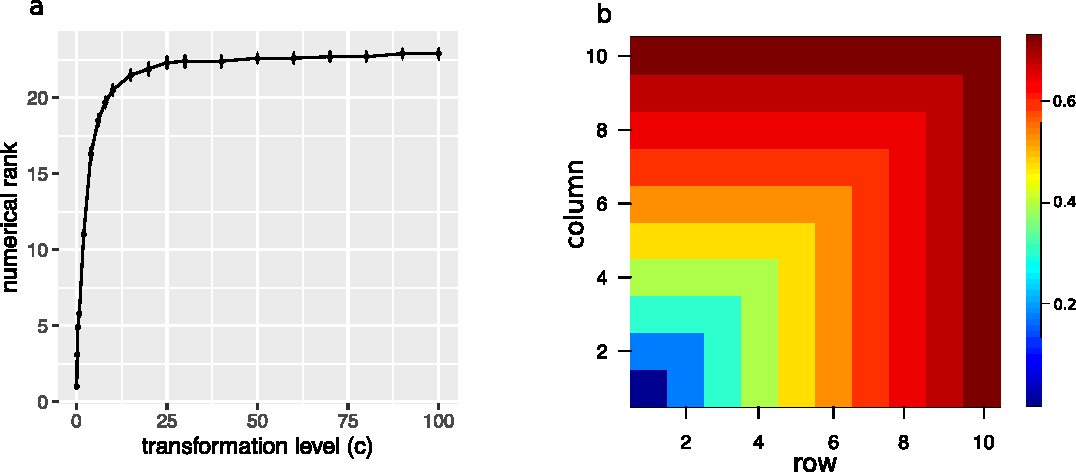
\includegraphics[width=.8\textwidth]{figure/low_rank.pdf}
\caption{Two examples of high-rank matrix trace model. (a) Numerical rank of the matrix $g(\mB)$ versus $c$ in the transformation, where the numerical rank is defined by $\rank(g(\mB))=\min\{\rank(\mC )\colon \FnormSize{}{\mC-g(\mB)} \leq 0.01 \FnormSize{}{g(\mB)} \}$. The error bar represents standard error from 10 realizations of $\mB$. (b) Heatmap of a full-rank matrix $\mB\in\mathbb{R}^{d\times d}$ with the $(i,j)$-th entry equal to $\log(1+\max(i,j))$. In (a), $d=50$, and in (b), $d=10$.} 
\label{fig:limit}
\label{penG}
\end{figure}

These examples reveal inadequacy of the conventional low-rank trace model~\eqref{eq:linear} in capturing important yet complicated matrix effects. This has motivated us to develop a new and flexible class of nonparametric trace regression models for capturing nonlinear, local, and possibly high-rank effects for high-dimensional matrices. We will revisit these two examples in Section~\ref{sec:idea} and show how these limitations can be avoided using a richer matrix model based on what we coin as the ``sign-rank'' of a matrix. 

%%%%%%%%%%%%%%%%%%%%%%%%%%%%%%%%%%%%%%%%%%%%%%
\subsection{Our proposal and contributions}

In this article, we propose a new notion of low-rank sign representable function, then develop a flexible class of nonparametric trace regression models built on this notion. Our proposal makes useful contributions to multiple fronts. 

First, we develop a new nonparametric regression paradigm -- structured sign representations -- that addresses the challenges previously difficult or infeasible in trace regressions, especially in the high-dimensional regime where $d_1d_2\gg n$. Existing literature on matrix regressions almost exclusively focuses on low-rank trace effects in the global scale. However, such a premise often fails, where the rank of global effects may grow with the matrix dimension. By contrast, our proposed model enjoys rank invariance under monotonic transformations, and permits both low-rank and high-rank effects through aggregation of sign representation functions. We show that the low-rank sign functions not only preserve all information for conventional low-rank models, but also bring additional flexibility and accuracy in more complicated nonlinear, high-rank models. As such, our framework is highly flexible, incorporates conventional low-rank matrix models, and is applicable to aforementioned high-rank matrix learning problems. The work fills a crucial gap between a global parametric model and a local nonparametric model, and enriches the matrix modeling literature. 

Second, we show that the sign function series can be statistically characterized by classification tasks with carefully specified weights. This characterization converts a complex and hard regression problem \emph{``what is the value of the nonparametric regression function?''} to a series of simpler and easier classification problems \emph{``does the regression function fall below a threshold?''} Correspondingly, we develop a learning reduction approach to estimate the regression function via a series of classifiers. This ability to import and leverage existing classification solutions is another advantage of our method. Theoretically, we establish the excess risk bounds, estimation error rates, and sample complexities. Particularly, our error bound reveals the well-controlled complexity from sign estimation to regression, where 
\begin{align*}
\text{sign function error }& \lesssim \KeepStyleUnderBrace{t_n^{\alpha/( 2+\alpha)}}_{\text{classification error}},\\
\text{regression error } & \lesssim  \KeepStyleUnderBrace{t_n^{\alpha/(2+\alpha)}}_{\text{estimation error inherited from classification}}+\KeepStyleUnderBrace{\textstyle{1\over H}}_{\text{reduction bias}}+\KeepStyleUnderBrace{Ht_n}_{\text{reduction variance}},
\end{align*}
in which $\alpha\geq 0$ quantifies the smoothness of the nonparametric regression function, $H\in\mathbb{N}_{+}$ is a resolution parameter that specifies the total number ($2H+1$) of sign functions to aggregate in our algorithm, $t_n=t_n(d,n)\to 0$ quantifies the convergence rate depending on the specific model, and $d=d_1=d_2$ for simplicity. In particular, we establish $t_n\asymp n^{-1}\log d$ under a two-way sparse non-parametric trace regression model (see Section~\ref{sec:sparse}) and $t_n \asymp n^{-1}d$ under a low-sign-rank non-parametric matrix completion model (see Section~\ref{sec:matrixcompletion}). These results imply that a low sample complexity with respect to the matrix dimension. Note that the sign function estimation reaches a faster $\tO(n^{-1})$ rate compared to the $\tO(n^{-1/2})$ regression rate when $\alpha= \infty$, which confirms our premise that sign estimation is easier than regression. To our knowledge, these statistical guarantees are among the first for the learning reduction approach in the context of nonparametric matrix regression. 

Lastly, we develop an alternating direction method of multipliers (ADMM) algorithm for optimization with a family of large-margin loss functions. The algorithm leverages recent advances in large-margin solvers as well as nonconvex optimization for low-rank two-way sparse matrix learning. We demonstrate that the proposed learning method enjoys both easy interpretability and accurate prediction through both simulations and real data applications. 



%%%%%%%%%%%%%%%%%%%%%%%%%%%%%%%%%%%%%%%%%%%%%%
\subsection{Related work}

Our work is related to but also clearly distinctive from several lines of existing research. We first comment that, nonparametric learning for matrix data is challenging. Naively turning a matrix into a vector then applying classical vector-based nonparametric methods can destroy rich structural information encoded in the matrix data. Moreover, most nonparametric methods rely on some notion of smoothness in a local neighborhood of the predictors. In the context of matrix regression, however, the predictor space is huge and is barely explored by the data with a limited sample size.  

The first line is the classical trace regression \citep{fan2019generalized,hamidi2019low}. The key difference is that the existing solutions all adopt a parametric model with a global low-rank structure. By contrast, our method is nonparametric, introduces low-rank sign representations, and extends the usual matrix rank with a new notion of sign-rank. As a result, our model permits both linear and nonlinear trace effects, and embraces both low and high matrix rank effects. 
 
The second line is the recent development of nonparametric methods with matrix-valued or tensor-valued data. In imaging analysis, convolution neural networks (CNNs) have been widely adopted as a nonparametric tool for prediction given matrix-valued images \citep{goodfellow2016deep}. In contrast, our proposal studies not only prediction, but also estimation and interpretability, with theoretical guarantees. We also numerically compare our method with CNN. Hao et al.~\citep{hao2019sparse} propose a sparse additive model with tensor predictors by extending the usual spline basis functions. Zhou et al.~\citep{zhou2020broadcasted} study tensor predictors as well and propose a broadcasting operation to introduce nonlinearity to individual tensor entries. Our nonparametric solution has broader implications than these approaches~\cite{hao2019sparse, zhou2020broadcasted} in estimating local low-rank effects. Our sign series representation of function bridges the gap between regression and classification in high dimensions, and naturally lends the problem to a learning reduction type solution. Moreover, although matrix can be viewed as a two-dimensional tensor, the problem of nonparametric learning for matrix data itself is more parsimonious and deserves a full investigation. We leave the counterpart problem for nonparametric tensor regression as future research. 

The third line is function sign estimation, which is in turn related to classification, or more generally, the level set estimation. The latter problem has a long history in statistics \citep{tsybakov1997nonparametric} and computational mathematics \citep{gibou2018review}. Particularly, Wang et al.~\cite{wang2008probability} propose a conditional probability estimation method based on support vector machines (SVMs), but their results are restricted to a fixed number of features and vector predictors only. Singh et al.~\cite{singh2009adaptive} propose a tree-based method for multiple sets extraction, but their goal is level set estimation instead of function estimation. None of those methods address the regression problem or high-dimensional matrix predictors. By contrast, we bridge the problems of level set estimation and nonparametric regression using low-rank sign series representations. Instead of constructing a point-wise function in the domain space, the sign representation partitions the domain space based on the function range. The benefit bears the analogy of Lebesgue versus Riemann integrals in functional analysis, in the sense that the neighborhood is determined by the range space instead of the domain space. The former approach is especially appealing for matrix regressions, where the range space is determined by a simple scalar response, whereas the domain space is huge and high-dimensional. 

%%%%%%%%%%%%%%%%%%%%%%%%%%%%%%%%%%%%%%%%%%%%%%
\subsection{Notation and organization}

We adopt the following notation throughout this article. Let $\tX \subset \mathbb{R}^{d_1\times d_2}$ denote the feature space equipped by some measure $\mathbb{P}_{\mX}$. For a function $f\colon \tX \to \mathbb{R}$, let $\sign f$ denote its sign function, i.e., $\sign f(\mX)=1$ if $f(\mX)>0$ and $\sign f(\mX)=-1$ otherwise. Let $\onenormSize{}{f}$ denote its $L_1$ norm, such that $\onenormSize{}{f}=\mathbb{E}|f(\mX)|$, where the expectation is taken with respect to $\mX \sim \mathbb{P}_{\mX}$. For a set $A \subset \tX$, let $\sign (\mX\in A)$ denote the sign function induced by $A$, i.e., a function taking value $1$ on the event $\{\mX\in A\}$ and $-1$ otherwise. Let $[n] = \{1,\ldots,n\}$, and $|\cdot|$ denote the cardinality. Let $\newnormSize{}{\cdot}_p$ denote the vector $p$-norm for $p\geq 0$. For a matrix $\mB \in \mathbb{R}^{d_1\times d_2}$, let $\mB_i$ denote its $i$-th row and $B_{ij}$ its $(i,j)$-th entry. Let $\newnormSize{}{\mB}_{p,q}$ denote the matrix $(p,q)$-norm such that $\newnormSize{}{\mB}_{p,q}=\newnormSize{}{\mb}_q$, where $\mb=(\newnormSize{}{\mB_1}_p,\ldots,\newnormSize{}{\mB_{d_1}}_p)^T\in\mathbb{R}^{d_1}$ consists of the $p$-norms for each row of $\mB$. In particular, $\newnormSize{}{\mB}_{1,0}=|\{i\in [d_1]\colon \mB_i\neq 0\}|$ denotes the number of non-zero rows in $\mB$. Let $\FnormSize{}{\mB}=\sqrt{\langle \mB, \mB \rangle}$ the matrix Frobenius norm, and $\mnormSize{}{\mB}=\max_{(i,j)}|B_{ij}|$ the matrix maximum norm. Moreover, an event $E$ is said to occur ``with high probability'' if $\mathbb{P}(E)$ tends to 1 as the matrix dimension $d_{\min} = \min(d_1,d_2)\to\infty$. Denote $a_n\asymp b_n$ if $c_1\leq \lim_{n\to \infty} a_n/b_n\leq c_2$ for some constants $c_1,c_2>0$, and denote $a_n\lesssim b_n$ if $\lim_{n\to\infty} a_n/b_n\leq c$ for some constant $c\geq 0$. Let $\tO(\cdot)$ denote the big-O notation, $\tilde \tO(\cdot)$ the variant that hides the logarithmic factors, and $\mathds{1}(\cdot)$ the indicator function. Whenever applicable, the basic arithmetic operators are applied to a matrix in an element-wise manner. 

The rest of the article is organized as follows. Section \ref{sec:idea} presents the low-rank sign representable functions and our nonparametric trace regression model. Section \ref{sec:bridge} develops the learning reduction approach through weighted classifications, and establishes statistical guarantees. Section \ref{sec:examples} specializes the general theory to two concrete learning problems, 
the low-rank sparse matrix predictor regression and the high-rank matrix completion. Section \ref{sec:estimation} studies large-margin-based estimation and develops an optimization algorithm. Section \ref{sec:simulation} presents the simulations, and Section \ref{sec:realdata} two real data applications. Section \ref{sec:discussion} concludes with a discussion. All technical proofs and additional results are relegated to the Supplementary Appendix. 





%%%%%%%%%%%%%%%%%%%%%%%%%%%%%%%%%%%%%%%%%%%%%%
\section{Nonparametric trace regression model}
\label{sec:idea}

In this section, we present our nonparametric trace regression model. Let $\mX\in\tX\subset \mathbb{R}^{d_1\times d_2}$ denote the matrix predictor, $Y\in\mathbb{R}$ the scalar response, and $\mathbb{P}_{\mX,Y}$ the joint probability distribution. We consider the model,
\begin{equation}\label{eq:model}
Y=f(\mX)+\varepsilon,
\end{equation}
where $f\colon\tX\mapsto \mathbb{R}$ is an unknown regression function of interest, and $\varepsilon$ is a mean-zero noise. For simplicity, we assume the noise is bounded; the extension to a sub-Gaussian noise is provided in Section~\ref{sec:sub-Gaussian} of the Appendix. In the main paper we assume the range of $Y$ is the bounded interval $[-1,1]$ for cleaner exposition. In addition, we allow a heterogeneous noise such that $\varepsilon$ may depend on $\mX$. Model \eqref{eq:model} therefore incorporates both continuous and binary-valued responses. For instance, it includes the binary regression where $Y$ is a $\{0,1\}$-label from a Bernoulli distribution, in which case, the noise variance depends on the mean, and the regression function $f$ represents the conditional probability, $f(\mX)=\mathbb{P}(Y=1|\mX)$. Our goal is to estimate the regression function $f(\mX)=\mathbb{E}(Y|\mX)$ based on $n$ i.i.d.\ training samples $(\mX_i,Y_i)_{i=1,\ldots,n}$. 

We next introduce the notion of the low-rank sign representable function, which is essential to bridge the usual global low-rank trace models to nonparametric local low-rank trace models. 

\begin{definition}[Rank-$r$ sign representable function] \label{def:caliF}
A function $f\colon \tX\mapsto[-1,1]$ is called $(r,\pi)$-sign representable, for a given level $\pi\in[-1,1]$ and a rank $r \in \mathbb{N}_{+}$, if the function $(f-\pi)$ has the same sign as a rank-$r$ trace function; that is,
\begin{equation} \label{eq:sign}
\sign(f(\mX)-\pi) = \sign(\langle \mX, \mB \rangle+b),\quad \text{for all }\mX\in\tX,
\end{equation}
where $\mB=\mB(\pi)$ is a rank-$r$ matrix, and $b=b(\pi)$ is the intercept. A function $f$ is called globally rank-$r$ sign representable, if $f$ is $(r,\pi)$-sign representable for all $\pi\in[-1,1]$. Let $\caliF(r)$ denote the rank-$r$ sign representable function family, and let $\Phi(r)=\{\phi\colon \mX\to \langle \mX, \mB \rangle+b\ \big|\ \text{rank}(\mB)\leq r, (\mB,b)\in\mathbb{R}^{d_1\times d_2}\times\mathbb{R}\}$ denote the rank-$r$ trace function family.
\end{definition}

Next, we show that \eqref{eq:model} and \eqref{eq:sign} together form a very general family of models that incorporate most existing matrix regression models, including the low-rank trace regression, single index models, and high-rank matrix completion model. 

\begin{example}[Generalized trace regression] The linear and generalized trace regression \cite{zhou2014regularized, wang2017generalized, fan2019generalized} imposes that $f(\mX)=g(\langle \mX, \mB \rangle)$ with a known link function $g$ and a rank-$r$ coefficient matrix $\mB$. By definition, $\sign(f(\mX)-\pi)=\sign(\langle \mX, \mB \rangle -g^{-1}(\pi))$ holds for every $\pi$ in the function range. Therefore, our model includes the generalized trace regression, i.e, $f \in \caliF(r)$. In particular, the usual trace model corresponds to the identity link $g$. More generally, any monotonic $g$ suffices, e.g., the logistic function $g(z)=(1+\exp(-z))^{-1}$, the arctangent function $g(z)={1/\pi}\arctan(z)+{1/2}$, the rectified linear unit (ReLU) function $g(z)=\max(0,z)$, and any inverse cumulative distribution function. %Moreover, we note that the function $f$ itself may not be well approximated by a low-rank trace function, as we have shown in Section~\ref{sec:limit}. 
%On the other hand, our model does not require to know $g$ a priori. 
\end{example}

\begin{example}[Single index regression model] 
The monotonic matrix predictor single index model \citep{balabdaoui2019least,ganti2017learning} assumes a similar form of regression function $f(\mX)=g^{}(\langle \mX, \mB\rangle)$ with a low-rank $\mB$ and a monotonic $g$, but the form of $g$ is unknown. By definition, our model family $\caliF(r)$ incorporates the single index model and does not require to know $g$ a priori. 
\end{example}

\begin{example}[Multivariate normal mixture]
The prospective model from matrix linear discriminant analysis \citep{hu2020matrix} considers a binary response $Y=\{0,1\}$, and assumes the matrix $\mX|Y$ follows a Gaussian mixture distribution, $\mX|\{Y=i\} = \mB_0 + \mB\times i + \mE_i$, $i=0,1$, where $\mB_0$ is an arbitrary baseline matrix, $\mB$ is a rank-$r$ matrix, and $(\mE_i)_{i=0,1}$ are two mutually independent noise matrices with i.i.d.\ standard normal entries. Our model incorporates this model, by noting that $f(\mX)=\mathbb{E}(Y|\mX)=\text{logistic}(\langle \mB, \mX \rangle+b)$ for some $b\in\mathbb{R}$, and thus $f\in \caliF(r)$. 
\end{example}

Definition \ref{def:caliF} leads to another notion, the matrix sign-rank, which is important for understanding our proposed model for matrix completion as a special nonparametric trace regression. Specifically, for a given matrix $\mTheta\in\mathbb{R}^{d_1\times d_2}$, define its sign-rank as: 
\begin{equation*}
\srank(\mTheta)=\min\big\{ \rank(\mTheta')\colon \sign(\mTheta')=\sign(\mTheta),\  \mTheta'\in\mathbb{R}^{d_1\times d_2} \big\}.
\end{equation*}
This concept is important in areas such as combinatorics \citep{cohn2013fast} and quantum mechanics \citep{de2003nondeterministic}. To better understand this notion and its relation to the proposed nonparametric trace regression, we consider model~\eqref{eq:sign} with the predictor space $\tX = \{\ma^T_i\mb_j\colon (i,j)\in[d_1]\times[d_2]\}$, and $\ma_i\in\mathbb{R}^{d_1}, \mb_j\in\mathbb{R}^{d_2}$ are the basis vectors. For matrix completion, a function $f$ over $\tX$ is equivalently represented by a $d_1$-by-$d_2$ signal matrix $\mTheta=\entry{f(\me^T_i\me_j)}$. Our proposed function family $\caliF(r)$ essentially defines a new family of structured matrices with a low sign-rank, as shown in the next proposition. 

\begin{proposition}[Sign-representable function over basis matrices]\label{prop:signbasis} Consider the predictor space $\tX=\{\ma^T_i\mb_j \colon (i,j)\in[d_1]\times[d_2]\}$. We represent a bounded function $f\colon \tX\to [-1,1]$ by its function values organized as a matrix $\mTheta=\entry{f(\ma^T_i\mb_j)} \in [-1,1]^{d_1\times d_2}$ for basis vectors $\ma_i\in\mathbb{R}^{d_1}, \mb_j\in\mathbb{R}^{d_2}$. If $f$ is rank-$r$ sign representable, then $\max_{\pi\in[-1,1]}\srank(\mTheta-\pi)\leq r+1$ (the constant 1 is due to the intercept in~\eqref{eq:sign}). Conversely, if $\max_{\pi\in[-1,1]}\srank(\mTheta-\pi)\leq r$, then $\mTheta$ defines a rank-$r$ sign representable function $f$. 
\end{proposition}

Define the sign-$r$ representable family for the signal matrix in matrix completion.  
\begin{align*}
\caliM(r)=\{\mTheta\colon \max_{\pi\in[-1,1]}\srank(\mTheta-\pi)\leq r, \ \mnormSize{}{\mTheta}\leq 1\}.
\end{align*}
The family $\caliM(r)$ is a special case of the function family $\caliF(r)$ in Definition \ref{def:caliF} with $b=0$ and the predictor space $\tX=\{\ma_i^T\mb_j\colon (i,j)\in[d_1]\times[d_2]\}$. We next further compare the sign-rank with the matrix rank in this setting. 

\begin{proposition}[Sign-rank vs. matrix rank]\label{prop:signrank} Consider the setting in Proposition \ref{prop:signbasis}. Then we have,
\begin{enumerate}[(a)]
\item $\max_{\pi\in[-1,1]}\srank(\mTheta-\pi)\leq \rank(\mTheta)+1$.
\item If $\mTheta \in \caliM(r)$, then $g(\mTheta)/\mnormSize{}{g(\mTheta)}\in\caliM(r+1)$ for any strictly monotonic function $g\colon \mathbb{R}\to\mathbb{R}$.
\item For every dimension $d$, there exists a $d$-by-$d$ matrix $\mTheta\in\caliM(2)$ such that $\rank(\mTheta)= d$.  
\end{enumerate}
\end{proposition}

\noindent
Proposition \ref{prop:signrank} highlights the advantages of using the sign-rank in the high-dimensional matrix analysis. The first property implies that classical low-rank matrix model is a special case of our low-sign-rank model. The second property shows that, compared to the matrix rank, the sign-rank remains nearly invariant under monotonic transformations, since $\srank(g(\mTheta)) \leq 1+\srank(\mTheta)$ for all monotonic functions $g$. The last property shows that the sign-rank can be dramatically smaller than the conventional matrix rank. Therefore, our model $\caliM(r)$ is strictly richer than the usual low-rank model. 

One key advantage about the sign-rank concept is that low-sign-rank assumptions are more relaxed and hence more realistic than classical low rankness assumptions. We next revisit the high-rank matrix model in Fig~\ref{fig:limit}(a) to show that $\mB$ is of a high matrix rank but a low sign-rank. Meanwhile, we provide some additional examples of low-sign-rank matrices in Section~\ref{sec:signrank} of the Appendix, including matrices from graphon models \cite{chan2014consistent}, banded matrices, and the identity matrix.

\begin{example}[Single index model-based matrix completion]
For the model in Fig~\ref{fig:limit}(a), $g(\mB)$ is a low-sign-rank matrix because $\srank(g(\mB)-\pi)\leq 1+\rank(\mB)=6$ for all $\pi$ in the function range. However, $g(\mB)$ itself is often high-rank as shown in Fig~\ref{fig:limit}(a).
\end{example}

\begin{example}[High-rank matrix completion model]\label{ex:high-rank}
For the model in Fig~\ref{fig:limit}(b), the matrix $\mB=\entry{\log(1+\max(i,j)/d)}$ is full-rank. Remarkably, this high-rank matrix belongs to our sign representable function with rank 2, i.e., $\mB\in \caliM(2)$. This is because $\srank(\mB-\pi)=\srank(\bar \mB)$, where $\bar \mB=\entry{\sign(\max(i,j)-e^\pi+1)}$ is a block matrix with rank at most 2. More generally, matrices of the type $\mB=\entry{g(\max(i,j)/d)}$ belong to $\caliM(2r)$, where $g(\cdot)$ is a polynomial of degree $r$.
\end{example}

Our proposed nonparametric matrix regression model $\caliF(r)$ therefore implies a new matrix completion model in $\caliM(r)$. In the sequel, we will establish the general theory for $\caliF(r)$ first, and then specialize the results to the specific high-rank completion setting in~\ref{sec:matrixcompletion}. 

%%%%%%%%%%%%%%%%%%%%%%%%%%%%%%%%%%%%%%%%%%%%%%
\section{From classification to regression: a learning reduction approach}
\label{sec:bridge}

In this section, we present a learning reduction approach to estimate $f$ from the model as specified in \eqref{eq:model} and \eqref{eq:sign}. Our main crux is to provably convert
the regression estimation problem into a series of sign function estimation problems, which are solved by weighted classifications. 

More specifically, we dichotomize the response $Y_i$ into a series of binary versions $\sign(Y_i-\pi)$ for $\pi\in\tH=\{-1,\ldots,-{1/H}, 0, {1/H}, \ldots,1\}$, where $H\in\mathbb{N}_{+}$ is a resolution parameter and $2H+1$ is the total number of sign functions. Then, for each $\pi$, we estimate the sign function $\sign(f-\pi)$ by performing a classification task, 
\begin{equation}\label{eq:proposal}
\hat \phi_\pi =\argmin_{\phi\in\Phi(r)}{1\over 2n}\sum_{i=1}^n\text{weighted-classification}(\sign(Y_i-\pi),\ \sign \phi(\mX_i)),
\end{equation}
where $\Phi(r)$ is the collection of rank-$r$ trace functions, and the weighted classification$(\cdot,\cdot)$ denotes a classification objective function with response-specific weight to each sample point. The weight in the objective function is crucial in our method, and we will detail the form in next section. Our final regression function estimate takes the form, 
\begin{equation}\label{eq:stepfunction}
\hat f= {1\over 2H+1}\sum_{\pi \in \tH} \sign \hat \phi_\pi.
\end{equation}
We comment that the $(2H+1)$ estimation tasks of the sign functions are fully separable, leading naturally to a parallel solution. Moreover, the sign functions bridge the problems of level set estimation and Bayes classification. Fig~\ref{fig:method} illustrates our main idea graphically. 

Next, we describe the specific form of weighted classification, the uniqueness of the classification optimizer, as well as the accuracy guarantee of the estimator. 

\begin{figure}[t!]
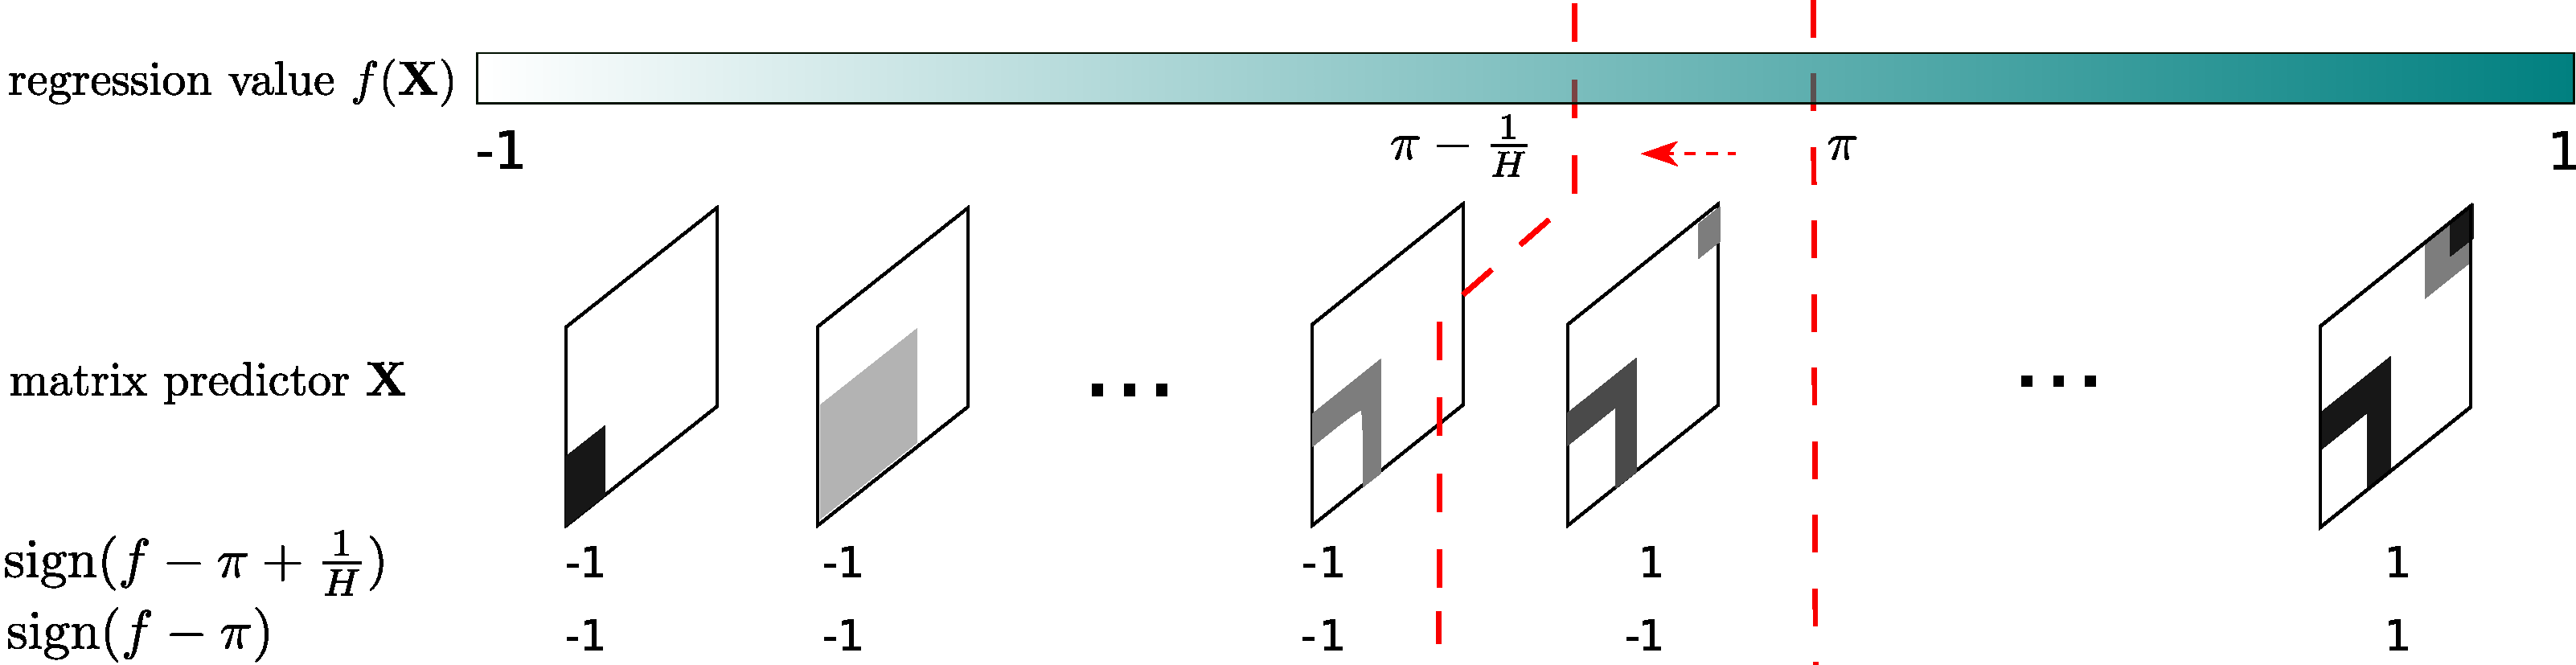
\includegraphics[width=\textwidth]{figure/demo_method.pdf}
\caption{Nonparametric matrix regression via sign function series estimation. We use a series of weighted classifications to estimate the sign functions, then obtain the regression function estimate via sign aggregation. Here, $\mX\in\tX$ denotes matrix-valued predictor, $f\colon \tX\to \mathbb{R}$ denotes regression function, and $\sign(f-\pi)\in\{-1,1\}$ is the sign function, where $\pi\in\{-1,\ldots,-1/H,0,1/H,\ldots, 1\}$ is the series of levels to aggregate in our algorithm.}
\label{fig:method}
\end{figure}



%%%%%%%%%%%%%%%%%%%%%%%%%%%%%%%%%%%%%%%%%%%%%%
\subsection{Statistical characterization of sign functions via weighted classification}

For a given level $\pi\in[-1,1]$, define the $\pi$-shifted response $\bar Y_{\pi,i} =Y_i-\pi$ for $i\in[n]$. We propose a weighted classification objective function in~\eqref{eq:proposal} using 
\begin{equation}\label{eq:loss}
L(\phi;(\mX_i,\bar Y_{\pi,i})_{i\in[n]})={1\over 2n}\sum_{i=1}^n\KeepStyleUnderBrace{|\bar Y_{\pi,i}|}_{\text{response-specific weight}}\times\KeepStyleUnderBrace{|\sign \bar Y_{\pi,i} - \sign \phi(\mX_i)|}_{\text{classification loss}},
\end{equation}
where $\phi\in \Phi(r)$ is the trace function to be optimized, and $|\bar Y_{\pi, i}|$ serves as the weight. Such a response-specific weight incorporates the magnitude information of responses into classification, in that the response values that are far away from the target level are penalized more heavily in the objective \eqref{eq:loss}. In the special case of a binary response $Y_i\in\{-1,1\}$ and target level $\pi=0$, the objective \eqref{eq:loss} reduces to the usual classification loss. 

Next, define the weighted classification risk, 
\begin{equation}\label{eq:constrained}
\risk_\pi(\phi)=\mathbb{E}L(\phi; (\mX_i,\bar Y_{\pi,i})_{i\in[n]}),
\end{equation}
where the expectation is taken with respect to the joint distribution of $(\mX_i,Y_i)$ i.i.d.\ from $\mathbb{P}_{\mX,Y}$. The next theorem quantifies the global optimum of \eqref{eq:constrained}. 

\begin{theorem}[Global optimum of weighted classification risk]\label{thm:oracle} For any given level $\pi\in[-1,1]$, under the model specified in \eqref{eq:model} and \eqref{eq:sign}, for all functions $\bar f$ that have the same sign as $\sign(f-\pi)$, it holds that $\risk_\pi(\bar f) = \inf\{\risk_\pi(\phi)\colon \phi\in \Phi(r)\}$. 
\end{theorem}

\noindent
Theorem~\ref{thm:oracle} suggests a practical procedure to estimate $\sign(f-\pi)$ through weighted classifications. It shows that the sign function $\sign(f-\pi)$ minimizes the weighted classification risk. The inverse, however, may not hold true, due to possible multiple global optimizers of $\risk_\pi(\cdot)$. A simple example is a constant regression $f(\mX)=\mathbb{E}(Y|\mX) = c$, in which case, every function $\phi\in \Phi$ minimizes $\risk_\pi(\cdot)$ at the level $\pi=c$. 



%%%%%%%%%%%%%%%%%%%%%%%%%%%%%%%%%%%%%%%%%%%%%%
\subsection{Identifiability}

To establish the statistical guarantee of the minimizer of $\risk(\cdot)$, we first address its uniqueness, up to some sign equivalence. It turns out the local behavior of the regression function $f$ around $\pi$ plays a key role to establish the identifiability of sign function series from weighted classifications.

We first introduce some additional notation. We call $\bayesS(\pi)=\{\mX\in\tX\colon f(\mX)\geq \pi\}$ the Bayes set at level $\pi$, and $\partial \bayesS(\pi)=\{\mX\in \tX\colon f(\mX)=\pi\}$ the level set boundary. Note that there is a one-to-one correspondence between the sign function $\sign(f-\pi)$ and the Bayes set $\bayesS(\pi)$. We choose to present the results in terms of $\bayesS(\pi)$ for easier comparison with the existing classification literature \citep{tsybakov2004optimal,singh2009adaptive}. We call a level $\pi\in[0,1]$ a mass point if the level set boundary $\partial \bayesS(\pi)$ has a non-zero measure under $\mathbb{P}_{\mX}$. Let $\tN=\{\pi\in[-1,1] \colon \mathbb{P}_{\mX}\left[f(\mX)=\pi\right]\neq 0\}$ denote the collection of all mass points in $f$. Suppose there exists a constant $c>0$, independent of the feature space dimension, such that $|\tN|\leq c<\infty$. 
We next introduce a notion of smoothness. The smoothness is described by the cumulative distribution function (CDF) of $f(\mX)$ under measure $ \mathbb{P}_{\mX}$, denoted as $G(\pi)=\mathbb{P}_{\mX}[f(\mX)\leq \pi]$.

\begin{definition} [$\alpha$-smoothness] \label{ass:decboundary} 
Suppose $\mathbb{P}_{\mX}$ is a continuous distribution. A function $f$ is called $(\alpha,\pi)$-locally smooth, for a given $\pi \notin \tN$, if there exist constants $C=C(\pi)>0$ and $\alpha=\alpha(\pi)\geq 0$, such that
\begin{equation}\label{eq:mass}
\sup_{0\leq t<\rho(\pi, \tN)}{G(\pi+t)-G(\pi-t)\over t^{\alpha}}\leq C,
\end{equation}
where $\rho(\pi,\tN) = \min_{\pi'\in \tN} |\pi-\pi'|$ denotes the distance from $\pi$ to the nearest point in $\tN$. We make the convention that $\rho(\pi,\tN)=2$, which equals the range of $\pi\in[-1,1]$ when $\tN$ is empty, and $\alpha=\infty$ when the numerator in \eqref{eq:mass} is zero. The largest possible $\alpha=\alpha(\pi)$ in \eqref{eq:mass} is called the smoothness index at level $\pi$. The function is called $\alpha$-globally smooth, if \eqref{eq:mass} holds with a global constant $C$ for all $\pi\in[-1,1]$ except for a finite number of levels.
\end{definition}

\noindent
Fig~\ref{fig:CDF} shows three examples of the CDF with various levels of smoothness. A small value of $\alpha<1$ indicates the infinite density at level $\pi$, or equivalently, when $G(\pi)$ jumps at $\pi$. A large value of $\alpha>1$ corresponds to the case of no point mass around $\pi$, or equivalently, when $G(\pi)$ remains flat. An intermediate case is $\alpha=1$ when $G(\pi)$ has a finite non-zero sub-derivative in the vicinity of $\pi$. The global smoothness index is the minimal $\alpha$ over all $\pi$'s; meanwhile, we allow exception for a finite number of levels. 

\begin{figure}
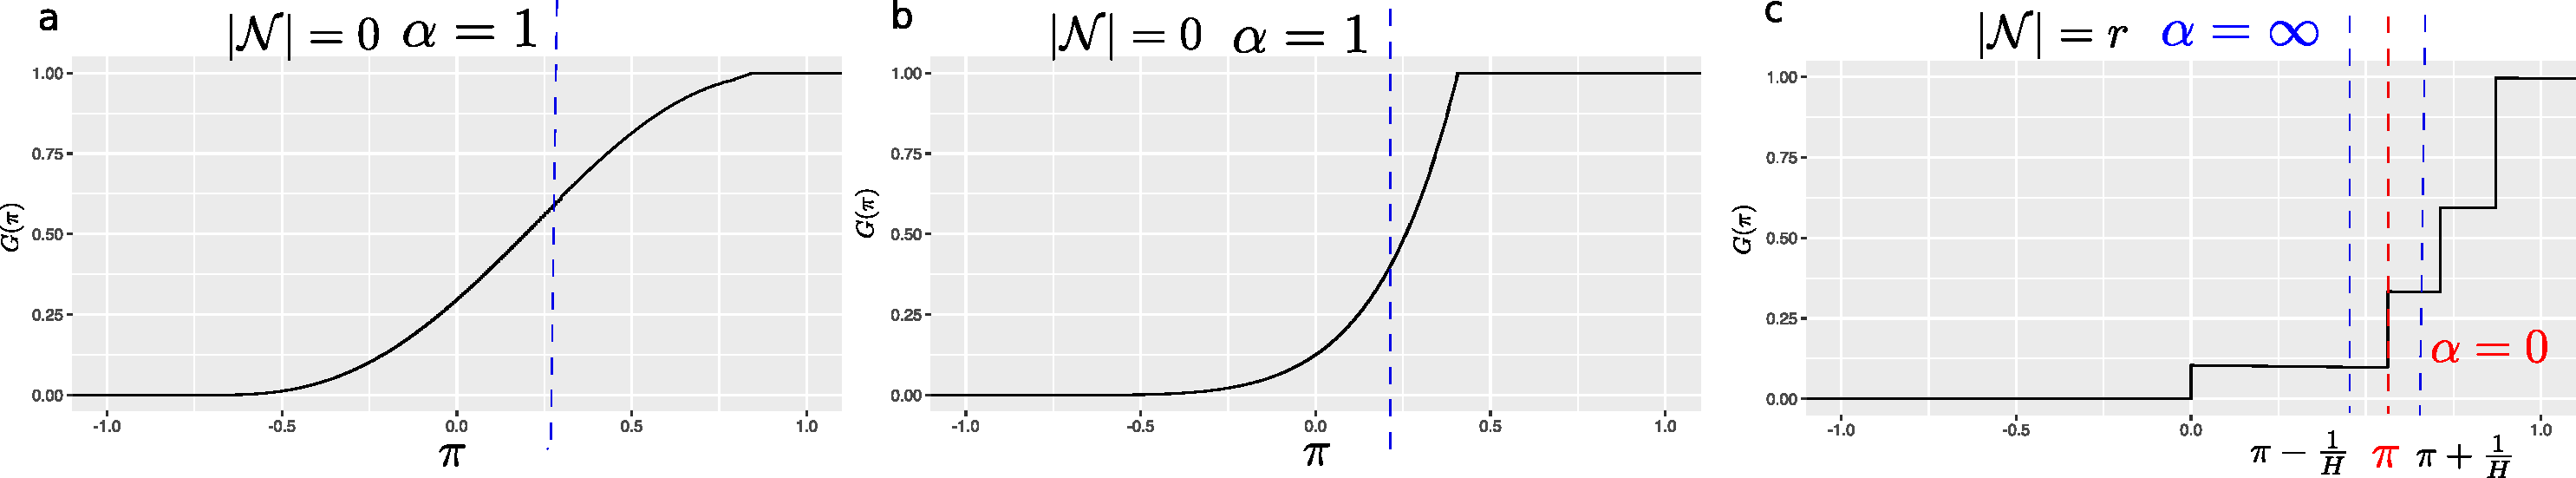
\includegraphics[width=.95\textwidth]{figure/cdf_new.pdf}
\caption{Three examples of CDF, $G(\pi)=\mathbb{P}_{\mX}(f(\mX)\leq \pi)$, with local smoothness index $\alpha$ at $\pi$ depicted in dashed line. (a) and (b). Function $G(\pi)$ $\alpha=1$ because the $G(\pi)$ has finite sub-derivatives in the range of $\pi$; (c). Function $G(\pi)$ with $\alpha=\infty$ at most $\pi$ (in blue), except for a total number of $|\tN|=r$ jump points (in red). Here $|\tN|$ denotes the number of jump points.}
\label{fig:CDF}
\end{figure}

Next, we show that the $\alpha$-smoothness with $\alpha\neq 0$ implies the uniqueness of $\bayesS(\pi)$ for the optimizer of $\risk(\cdot)$. For two sets $S_1, S_2\in \tX$, define the probabilistic set difference, 
\begin{align*} %\label{eq:riskdiff}
d_{\Delta}(S_1,S_2) = \mathbb{P}_{\mX}(S_1\Delta S_2)=\mathbb{P}_{\mX}\{\mX\colon \mX\in S_1\setminus S_2 \text{ or }S_2\setminus S_1\},
\end{align*}
and the risk difference,
\begin{align*} %\label{eq:setdiff}
d_\pi(S_1,S_2) = \risk_\pi(\sign(S_1))-\risk_\pi(\sign(S_2)).
\end{align*}

\begin{theorem}[Identifiability]~\label{thm:identifiability} Suppose $f$ is $\alpha$-globally smooth over $\tX$. Then,
\begin{align}\label{eq:identity}
d_{\Delta}(S,\bayesS(\pi)) \lesssim \left[d_\pi(S,\bayesS(\pi))\right]^{\alpha\over 1+\alpha}+{1\over\rho(\pi, \tN)} d_\pi(S,\bayesS(\pi)),
\end{align}
for all sets $S\in\tX$ and all levels $\pi\in[-1,1]$ except for a finite number of levels.
\end{theorem}

\noindent
We make two remarks. First, the bound~\eqref{eq:identity} controls the worst-case perturbation of the classifiers under the measure $\mathbb{P}_{\mX}$ with respect to the weighted classification risks. When $\alpha \neq 0$, the inequality \eqref{eq:identity} immediately implies the uniqueness, up to a measure-zero set in $\mathbb{P}_{\mX}$, of $\bayesS(\pi)$ in minimizing $\risk_\pi(\cdot)$. Second, our identifiability improves the earlier results for a single level set estimation to multiple level set estimations. Existing work \citep{singh2009adaptive,xu2020class} considered only a fixed number of $\pi$'s, and provided only the first term in the bound \eqref{eq:identity}. In contrast, our bound quantifies the full dependence on the level $\pi$, and establishes the recovery condition of $\bayesS(\pi)$ uniformly over all possible $\pi$'s. It turns out both terms in the bound \eqref{eq:identity} are crucial for our regression function estimation. The first term contributes to the classification error, and the second term contributes to the variance in sign series aggregation. 



%%%%%%%%%%%%%%%%%%%%%%%%%%%%%%%%%%%%%%%%%%%%%%
\subsection{Regression risk bound}

In this section, we provide the statistical accuracy guarantee for the learning reduction based estimation~\eqref{eq:proposal} and~\eqref{eq:stepfunction}. Our theory consists of three main ingredients. We first leverage the $\alpha$-smoothness to provide a sharp rate for $\hat \phi_\pi$'s classification risk than the usual root-$n$ convergence. The improvement stems from the fact that, under considered assumptions, the variance of the excess classification loss is bounded in terms of its expectation. Because the variance decreases as we approach the optimal $\sign(f-\pi)$, the risk of $\hat \phi_\pi$ converges more quickly to the optimal risk than the simple uniform converge results would suggest.  The second step is to convert the risk error into probability set error by Theorem~\ref{thm:identifiability}. The last step is to aggregate the set errors into the final nonparametric function estimation. A careful error analysis reveals the joint contribution from sign aggregation and variance-bias trade-off. 

The following result shows the estimation accuracy for sign function estimate \eqref{eq:proposal}. 
\begin{theorem}[Sign function estimation]\label{thm:main} Suppose the regression function $f\in\caliF(r)$ is $\alpha$-globally smooth over $\tX$, and let $d_{\max}=\max(d_1,d_2)$. Then, for all $\pi\in[-1,1]$ except for a finite number of levels, with high probability at least $1-c\exp(-rd_{\max})$ over the training data $(\mX_i,Y_i)_{i\in[n]}$, we have, 
\begin{equation}\label{eq:riskbound}
\onenormSize{}{\sign \hat \phi_\pi- \sign(f-\pi)} \lesssim \left({rd_{\max} \over n}\right)^{\alpha\over 2+\alpha}+{1\over \rho^2(\pi, \tN)}\left({rd_{\max}\over n}\right),
\end{equation}
where the $L_1$ norm is taken with respect to the measure $\mX\sim\mathbb{P}_{\mX}$ and $c>0$ is a constant. 
\end{theorem}

\noindent
Theorem~\ref{thm:main} quantifies the statistical convergence of sign function estimation. For a fixed $\pi$, the second term in \eqref{eq:riskbound} is absorbed into the first term, leading to the rate $O(n^{-\alpha/(2+\alpha)})$. We find that the sign estimation reaches a fast rate $1/n$ when $\alpha =\infty$, but has a slower rate when point mass concentrates with $\alpha=0$. This is consistent with our intuition, because $\alpha = \infty$ corresponds to a clear separation with no point mass at the Bayes set boundary $\partial \bayesS(\pi)$, whereas the worst rate $\alpha = 0$ corresponds to a heavy mass around $\partial \bayesS(\pi)$. Furthermore, the sign function estimation achieves consistency in the high-dimensional region as long as $n \gg d_{\max}\to \infty$ and $\alpha\neq 0$. Combining the sign representability of the regression function and the sign estimation accuracy, we obtain our main theoretical result on nonparametric trace regression. 

\begin{theorem}[Regression function estimation]\label{thm:regression} 
Suppose the same conditions in Theorem~\ref{thm:main} hold. With high probability at least $1-c\exp(-rd_{\max})$ over the training data $(\mX_i,Y_i)_{i\in[n]}$, we have 
\begin{align}\label{eq:bound}
\onenormSize{}{\hat f-f} \lesssim \KeepStyleUnderBrace{\left({rd_{\max}\over n}\right)^{\alpha \over 2+\alpha}\log H}_{\text{estimation error from sign functions}}+\KeepStyleUnderBrace{1\over H}_{\text{reduction bias}}+\KeepStyleUnderBrace{\left({rd_{\max}\over n}\right)H\log H}_{\text{reduction variance}},
\end{align}
for any resolution parameter $H \in \mathbb{N}_{+}$. In particular, setting $H\asymp \left( {n\over rd_{\max}} \right)^{1/2}$ gives 
\begin{equation}\label{eq:final}
\onenormSize{}{\hat f-f} \lesssim \tilde\tO \left\{ \left({rd_{\max} \over n}\right)^{\min\left({\alpha\over 2+\alpha}, {1\over 2}\right)}\right\},
\end{equation}
where the $L_1$ norm is taken with respect to the measure $\mX\sim\mathbb{P}_{\mX}$ and $\tilde \tO$ suppresses the log term. 
\end{theorem}

\noindent
Theorem~\ref{thm:regression} establishes the convergence rate of the proposed learning reduction estimator for nonparametric trace regression. We make three remarks. First, the bound~\eqref{eq:bound} reveals three sources of errors: the estimation error from sign functions, the bias due to sign series representations, and the variance thereof. Recall that $H$ determines the number of sign functions in sign series representations. It controls the bias-variance tradeoff here. Second, the regression is robust to a few off-target classifications, as long as the majorities are accurate. This can also be seen in Fig~\ref{fig:CDF}(a) where the classification is nonidentifiable at some mass point (red line). Nevertheless, regression estimation is still possible because the nearby classifications provide the sign signal (blue lines). This fact shows the benefit of sign aggregation, and also explains the trade-off in choosing $H$. Intuitively, a larger value of $H$ increases the approximation accuracy, meanwhile renders the classification harder near the mass points. Third, the final regression error is generally no better than the sign error, when we compare the bounds in \eqref{eq:final} with \eqref{eq:riskbound}. This confirms our earlier premise that classification is easier than regression. On the other hand, our sign representation approach allows us to disentangle the complexity and achieve the theoretical guarantee from classification to regression.


%%%%%%%%%%%%%%%%%%%%%%%%%%%%%%%%%%%%%%%%%%%%%%
\section{Two applications of nonparametric matrix learning}
\label{sec:examples}

In this section, we apply the general theory in Theorem~\ref{thm:regression} to two specific nonparametric matrix learning problems, the low-rank sparse matrix predictor regression, and the high-rank matrix completion. 



%%%%%%%%%%%%%%%%%%%%%%%%%%%%%%%%%%%%%%%%%%%%%%
\subsection{Low-rank sparse matrix predictor regression}
\label{sec:sparse}

The first problem we consider is matrix predictor regression. In addition to the low-sign-rank structure, we also introduce a two-way sparsity structure. That is, we impose that some rows and columns of $\mB$ are zeros, where $\mB$ is as defined in \eqref{eq:sign}. We comment that sparsity is a commonly used structure in matrix data modeling \citep{zhou2014regularized}, and in particular, this assumption is scientifically reasonable in brain connectivity applications \citep{Zhang2015}.

Specifically, we extend the notation $\Phi(r)$ and $\caliF(r)$ introduced in Definition~\ref{def:caliF} to incorporate the sparsity. Let $\Phi(r,s_1,s_2)$ denote the collection of trace functions, 
\begin{align*} %\label{eq:class}
\Phi(r,s_1,s_2)=\{\phi\colon \mX\mapsto \langle \mX, \mB \rangle +b \ \big| \text{rank}(\mB)\leq r,  \text{supp}(\mB)\leq (s_1,s_2), (\mB,b)\in\mathbb{R}^{d_1\times d_2}\times \mathbb{R}\},
\end{align*}
where $\text{supp}(\mB)$ denotes the support of $\mB$, with the sparsity parameters, $s_1=\newnormSize{}{\mB}_{1,0}=|\{i\in[d_1]\colon \mB_i\neq \mathbf{0}\}|$, and $s_2=\newnormSize{}{\mB^T}_{1,0}=|\{j\in[d_2]\colon \mB^T_j\neq \mathbf{0}\}|$, denoting the number of non-zero rows and non-zero columns of $\mB$, respectively. Similarly, let $\caliF(r,s_1,s_2)$ denote a family of rank-$r$, support-$(s_1,s_2)$ sign representable functions based on \eqref{eq:sign}. We have the following result. 

\begin{theorem}[Nonparametric low-rank two-way sparse regression]\label{thm:sparse}
Consider the same setup as in Theorem~\ref{thm:regression}, except that we replace $\caliF(r)$ and $\Phi(r)$ with $\caliF(r,s_1,s_2)$ and $\Phi(r,s_1,s_2)$, respectively. Set $H\asymp {\left(n\over r(s_1+s_2)\log d_{\max}\right)}^{1/2}$ in~\eqref{eq:stepfunction}. With high probability over the training data $(\mX_i, Y_i)_{i\in[n]}$, the estimate \eqref{eq:stepfunction} is bounded by
\begin{equation}\label{eq:final2}
\onenormSize{}{\hat f- f} \lesssim \tilde \tO\left\{\left({r(s_1+s_2)\log d_{\max} \over n}\right)^{\min\left({\alpha\over 2+\alpha}, {1\over 2}\right)}\right\}.
\end{equation}
\end{theorem}

\noindent
We make some remarks. First, the bound \eqref{eq:final2} suggests that the estimator remains consistent in the high-dimensional regime as $d_{\max}$ and $n\to \infty$, as long as $d_{\max}$ grows sub-exponentially in the sample size $n$. Such a sample complexity shows the pronounced advantage of the low-rank two-way sparse structural model, by comparing \eqref{eq:final2} and \eqref{eq:final}. Second, the two-way sparsity structure facilitates the interpretability, which we further demonstrate through numerical examples later. 



%%%%%%%%%%%%%%%%%%%%%%%%%%%%%%%%%%%%%%%%%%%%%%
\subsection{High-rank matrix completion}\label{sec:matrixcompletion}

The second problem we consider is matrix completion. Let $\mY\in\mathbb{R}^{d_1\times d_2}$ be a data matrix generated from the model,
\begin{equation}\label{eq:modelcompletion}
\mY=\mTheta+\mE,
\end{equation}
where $\mTheta\in\caliM(r)$ denotes an unknown signal matrix, and $\mE$ is an error matrix consisting of zero-mean, independent but not necessarily identically distributed entries. For simplicity, we assume $d_1=d_2=d$. Model \eqref{eq:modelcompletion} can be viewed as a special case of model \eqref{sec:idea}, where the predictor space consists of the basis matrices in $\mathbb{R}^{d\times d}$, and the data matrix $\mY=\entry{Y_{ij}}$ collects the scalar response $Y_{ij} \in \mathbb{R}$. In this case, the problem of regression estimation becomes the estimation of $\mTheta$. What is observed is an incomplete data matrix $\mY_\Omega$ from \eqref{eq:modelcompletion}, where $\Omega \subset [d]^2$ represents the index set of the observed entries. We allow both uniform and non-uniform sampling schemes for $\Omega$. Let $\Pi=\{p_\omega\}$ be an arbitrarily predefined probability distribution over the full index set with $\sum_{\omega\in[d]^2}p_\omega=1$. Assume the entries $\omega$ in $\Omega$ are i.i.d.\ draws with replacement from the full index set following the distribution $\Pi$. Denote the sampling rule as $\omega \sim \Pi$, and $\mY(\omega)$ the matrix entry indexed by $\omega$.  

Now applying our learning reduction approach to matrix completion problem~\eqref{eq:modelcompletion} yields the signal matrix estimate
\begin{equation}\label{eq:est}
\hat \mTheta = {1\over 2H+1}\sum_{\pi \in \tH}\sign(\hat \mZ_\pi),
\end{equation}
where, for every $\pi\in\{-1,\ldots,-1/H,0,1/H,\ldots,1\}$, the matrix $\hat \mZ_\pi$ is the solution to the weighted classification
\begin{equation*}
\hat \mZ_\pi = \argmin_{\mZ\colon \rank(\mZ)\leq r}\sum_{\omega\in\Omega} \KeepStyleUnderBrace{|\mY(\omega)-\pi|}_{\text{weight}}\KeepStyleUnderBrace{|\sign(\mY(\omega)-\pi)-\sign(\mZ(\omega))|}_{\text{classification loss}}.
\end{equation*}

\noindent
To assess the accuracy of the estimate $\hat \mTheta=\hat \mTheta_{d\times d}$ in the high dimensional regime $d\to \infty$, we need to put the model in the nonparametric context of Definition~\ref{ass:decboundary}. We now extend the notion of $\alpha$-smoothness to discrete feature space as follows. Let $\Delta s = 1/d^2$ denote a small tolerance, where $d^2$ represents the number of elements in the feature space. We quantify distribution of entries in matrix $\mTheta$ using pseudo density (a.k.a. histogram with bin width $2\Delta s$). Specifically, let $G(\pi)=\mathbb{P}_{\omega\sim \Pi}[\mTheta(\omega)\leq \pi]$ denote the CDF of $\mTheta(\omega)$ under $\omega\sim \Pi$. We partition $[-1,1]=\tN \cup \tN^c$, where $\tN$ consists of levels whose pseudo density based on $2\Delta s$-bin is asymptotically unbounded; i.e,
\[
\tN=\left\{\pi\in[-1,1] \colon {G(\pi+{\Delta s})-G(\pi-{\Delta s})\over \Delta s} \geq c_1 \right\},\ \text{for some universal constant }c_1>0,
\]
and $\tN^c$ otherwise. Let $|\tN|_{\text{cover}}$ be the covering number of $\tN$ with $2\Delta s$-bin's; i.e, $|\tN|_{\text{cover}} =\text{Leb}(\tN)/2\Delta s$, where $\text{Leb}(\cdot)$ denotes the Lebesgue measure. 

\begin{definition}[$\alpha$-smoothness for discrete distribution] Let $\Pi$ be the sampling distribution over $[d^2]$. We say the signal matrix $\mTheta(\omega)$ is $\alpha$-(globally) smooth under $\omega\sim \Pi$, if there exist constants $c_2,c_3>0$, such that $|\tN|_{\text{cover}}\leq c_2$ and
\begin{equation}\label{eq:smooth}
\sup_{\Delta s \leq t<\rho(\pi, \tN)}{G(\pi+{t})-G(\pi-{t})\over t^\alpha} \leq c_3, \quad \text{for all }\pi \in\tN^c,
\end{equation}
where $\rho(\pi,\tN)=\min_{\pi'\in \tN}|\pi-\pi'|+\Delta s$ denotes the adjusted distance from $\pi$ to the nearest point in $\tN$. 
\end{definition}
We assess the estimation error of~\eqref{eq:est} using mean absolute error (MAE), $\text{MAE}(\hat \mTheta, \mTheta)\stackrel{\text{def}}{=}\mathbb{E}|\hat \mTheta(\omega)-\mTheta(\omega)|$, where the expectation is take with respect to a future observation $\mTheta(\omega)$ from the distribution $G$.  We have the following result. 

\begin{theorem}[Nonparametric matrix completion]\label{thm:estimation} 
Consider the matrix model~\eqref{eq:modelcompletion} with $\alpha$-smooth signal matrix $\mTheta\in\caliM(r)$. Set $H \asymp \left( |\Omega|\over dr\right)^{1/2}$. With high probability over $\mY_\Omega$, the estimate \eqref{eq:est} satisfies that
\begin{equation}\label{eq:real}
\textup{MAE}(\hat \mTheta, \mTheta)\lesssim \tilde \tO\left\{\left(dr \over |\Omega|\right)^{\min({\alpha \over 2+\alpha}, {1\over 2})}\right\}.
\end{equation}
\end{theorem}

\noindent
We remark that our estimation accuracy \eqref{eq:real} applies to both low-rank and high-rank signal matrices. Moreover, the estimation rate depends on the sign complexity $\mTheta\in\caliM(r)$, where $r$ can be much smaller than the usual matrix rank as shown in Proposition \ref{prop:signrank}. In fact, our theorem can also be relaxed for growing $|\tN|_{\text{cover}}$ as a function of $d$, with slight modification on the setup (see Appendix~\ref{sec:unbounded} for extension). We now illustrate Theorem \ref{thm:estimation} with two matrix completion examples and compare with the existing literature.  

\begin{example}[Stochastic block model-based matrix completion]
The stochastic block model \cite{chi2020provable} assumes a checkerboard structure under marginal row and column permutations. The signal matrix belongs to our sign representable family $\mTheta \in \caliM(r)$, where $r$ is the total number of blocks. Furthermore, the block matrix is $\infty$-globally smooth, because $\tN$ consists of finitely many $2\Delta s$-bin's covering the block means in $\Theta$. Our signal estimate achieves the rate $\tilde\tO(d^{-1/2})$ when $\alpha=\infty$ in the absence of missingness. This rate agrees with the minimax root-mean-square error (RMSE) rate for stochastic block models with a fixed number of blocks \cite{gao2016optimal}. 
\end{example}

\begin{example}[Single index model-based matrix completion]
The single index model-based completion \cite{ganti2015matrix} admits a signal matrix $\mTheta=g(\mB)$, where $g$ is an unknown monotonic function, and $\mB$ is an unknown low-rank matrix. Note that the $\mTheta$ itself is often of a high matrix rank as shown in Fig~\ref{fig:limit}(a). Suppose the CDF of $\mTheta(\omega)$ has bounded psudo density with $\alpha=1$. Applying Theorem~\ref{thm:estimation} yields the estimation error rate $\tilde \tO(d^{-1/3})$, which is faster compared to the RMSE rate $\tilde \tO(d^{-1/4})$ obtained by \cite{ganti2015matrix}. 
\end{example}

Finally, we obtain the sample complexity of nonparametric matrix completion, summarized in the next corollary.

\begin{corollary}[Sample complexity for nonparametric completion] \label{thm:sample-complexity}
Suppose the same conditions of Theorem~\ref{thm:estimation} hold. When $\alpha\neq 0$, with high probability over $\tY_\Omega$, 
\begin{equation*}
\textup{MAE}(\hat \mTheta, \mTheta)\to 0, \quad \text{as}\quad {|\Omega|\over {d} r}\to \infty.
\end{equation*}
\end{corollary}

\noindent
Corollary \ref{thm:sample-complexity} improves earlier work~\cite{yuan2016tensor, pmlr-v119-lee20i} by allowing both low-rank and high-rank signals. Moreover, the sample size requirement depends only on the sign complexity $\tilde \tO(dr)$, but not the nonparametric complexity $\alpha$. We also note that $\tilde \tO(dr)$ roughly matches the degree of freedom of the signals, suggesting the optimality of our sample requirements.





%%%%%%%%%%%%%%%%%%%%%%%%%%%%%%%%%%%%%%%%%%%%%%
\section{Large-margin implementation and ADMM algorithm}
\label{sec:estimation}

In Section \ref{sec:bridge}, we have established the methodology and theory for nonparametric matrix trace regression under a 0-1 loss, since this is the canonical loss for classification. However, this loss is difficult to optimize. In this section, we replace the 0-1 loss with a continuous loss of a large-margin type, and present the corresponding optimization algorithm. We consider two large-margin loss functions: hinge loss $F(z) = (1-z)_+$ for support vector machines, and psi-loss $F(z)=2\min(1,(1-z)_+)$ with $z_{+}=\max(z,0)$~\cite{shen2003psi}. These two losses are most commonly used in classifications, and both satisfy linear excess risk bound (see Section~\ref{sec:large-margin}). 



%%%%%%%%%%%%%%%%%%%%%%%%%%%%%%%%%%%%%%%%%%%%%%
\subsection{Large-margin learning} 

We focus on nonparametric low-rank sparse matrix regression problems. With some straightforward modification, the solution applies to matrix completion and other matrix learning problems as well. Specifically, we generalize the 0-1 loss minimization \eqref{eq:loss} to the following minimization problem, 
\begin{align}\label{eq:large-margin}
\hat \phi_{\pi, F} = \argmin_{\phi \in\Phi(r,s_1,s_2)}\left\{ {1\over n}\sum_{i=1}^n |Y_i-\pi|F(\sign(Y_i-\pi)\phi(\mX_i))+ \lambda \FnormSize{}{\phi}^2\right\},
\end{align}
where $F(z)\colon \mathbb{R}\mapsto \mathbb{R}_{\geq 0}$ is a continuous function of the margin $z=y\phi(\mX)$, $\lambda>0$ is the penalty parameter, and $\FnormSize{}{\phi}$ is the penalty function. We set $\FnormSize{}{\phi}=\FnormSize{}{\mB}$, with $\mB$ being the coefficient matrix associated with $\phi\in\Phi(r,s_1,s_2)$. The use of large-margin loss in \eqref{eq:large-margin} allows us to leverage efficient large-margin optimization algorithms, while maintaining desirable statistical properties under mild conditions. The benefit of ridge penalization has been studied \cite{shen2003psi}. We obtain the corresponding regression function estimate as, 
\begin{equation}\label{eq:stepfunction-large-margin}
\hat f_{F} = {1\over 2H+1}\sum_{\pi \in \tH} \sign \hat \phi_{\pi, F}.
\end{equation}



%%%%%%%%%%%%%%%%%%%%%%%%%%%%%%%%%%%%%%%%%%%%%%
\subsection{ADMM optimization}

We next present an algorithm to solve \eqref{eq:large-margin} for a given $\pi\in\tH$. We first note that the estimation problem \eqref{eq:large-margin} is equivalent to the optimization,
\begin{equation}\label{eq:sampleoptim}
\min_{\substack{(\mB,b)\colon  \rank(\mB)\leq r, \text{supp}(\mB)\leq (s_1,s_2)}}{1\over n}\sum_{i=1}^n|\bar Y_{\pi, i}| F\left( \sign \bar Y_{\pi, i}[\langle \mX_i,\mB \rangle+b] \right) + \lambda\FnormSize{}{\mB}^2,
\end{equation}
where we recall $\bar Y_{\pi, i}=Y_i-\pi$ is the $\pi$-shifted response. The loss function $F$ can be convex, e.g., hinge loss, or non-convex, e.g., psi-loss. Meanwhile, the optimization \eqref{eq:sampleoptim} has a non-convex feasible region because of the low-rank and sparsity constraints. 

We propose an alternating direction method of multipliers (ADMM) algorithm to solve \eqref{eq:sampleoptim}. We introduce a dual variable and an additional feasibility constraint to perform coordinate descent in the augmented Lagrangian function. The augmented objective of \eqref{eq:sampleoptim} is
\begin{equation*} \label{eq:ADMM}
L(\mB,b, \mS,\mLambda,\rho) = {1\over n}\sum_{i=1}^n|\bar Y_{\pi, i}|F(\sign \bar Y_{\pi, i}[\langle \mX_i,\mB \rangle+b])  + \lambda\FnormSize{}{\mB}^2+\rho\FnormSize{}{\mB-\mS}^2+\langle \mLambda, \mB-\mS\rangle,
\end{equation*}
where $\mB\in \mathbb{R}^{d_1\times d_2}$ is the unconstrained primal variable, $\mS\in\mathbb{R}^{d_1\times d_2}$ is the constrained dual variable satisfying $\rank(\mS)\leq r$ and $\text{supp}(\mS)\leq (s_1,s_2)$, $\mLambda\in\mathbb{R}^{d_1\times d_2}$ is the Lagrangian multiplier, and $\rho>0$ is the step size parameter. Note that in $L(\mB,b, \mS,\mLambda,\rho)$, the non-convexity has moved from the first two terms in $\mB$ to the last two simpler terms in $\mS$. This separability simplifies the optimization for a wide range of loss functions and constraints. 

We next minimize $L(\mB,b, \mS,\mLambda,\rho)$ via coordinate descent, by iteratively updating one variable at a time while holding others fixed. Each update reduces to a simpler problem and can be efficiently solved by standard algorithms. 

Specifically, given variables $(\mS,\mLambda,\rho)$ and $\bar \mS = (2\rho\mS-\mLambda) / [2(\rho+\lambda)]$, the objective with respect to $(\mB,b)$ is 
\begin{equation*} \label{eq:primal}
L(\mB,b|\mS,\mLambda,\rho)={1\over n}\sum_{i=1}^n |\bar Y_{\pi, i}| F(\sign \bar Y_{\pi, i}[\langle \mX_i,\mB \rangle+b]) +(\lambda+\rho)\FnormSize{}{\mB-\bar \mS}^2.
\end{equation*}
Optimization with~\eqref{eq:primal} is a standard vector-based classification problem with a ridge penalty and an offset $\bar \mS$. There are a number of state-of-art algorithms for weighted SVM~\cite{wang2008probability} and psi-learning~\cite{shen2003psi}, which are readily available to solve this problem.  

Next, given $(\mB,b,\mLambda,\rho)$, and $\bar \mB=(2\rho\mB+\mLambda) / (2\rho)$, the objective with respect to $\mS$ is
\begin{equation}\label{eq:dual}
L(\mS|\mB,b,\mLambda,\rho)=\FnormSize{}{\mS-\bar \mB}^2,\quad \text{subject to} ~~ \rank(\mS)\leq r \text{ and }\text{supp}(\mS)\leq (s_1,s_2).
\end{equation}
This is equivalent to the best sparse low-rank approximation, in the least-square sense, to the matrix $\mB$. Compared to the original objective~\eqref{eq:sampleoptim}, the least-square objective is easier to handle. A number of learning methods and algorithms have been designed to solve this problem, e.g., sparse PCA, sparse SVD, and projection pursuit \citep{Ma2013}. We adopt the recently developed double projection method, which has a competitive performance in the high-dimensional regime \cite{yang2016rate}. 

Finally, the Lagrangian multiplier $\mLambda$ is updated by $\mLambda\leftarrow\mLambda+2\rho(\mB-\mS)$. Following some common practice in matrix nonconvex optimization \citep{yang2016rate}, we run the optimization from multiple initializations to locate a final estimate with the lowest objective value. We summarize the above optimization procedure in Algorithm \ref{alg:weighted}. 


\subsection{Hyperparameter tuning}
We briefly describe the hyperparameters in our Algorithm~\ref{alg:weighted}. Our method consists of two sets of hyperparameters, one for model specification, and another for algorithmic stability. The main model hyperparameters are $(r,s_1,s_2)$, which determine the complexity of sign functions. In practice, we choose $(r,s_1,s_2)$ via a grid search using cross validation based on regression error. The  resolution in grid search depends on the problem size; for example, in our brain connectivity data with $d_1=d_2=68$ (Section~\ref{sec:brain}), we search $r, s_1,s_2$ over $[d]$, with increment of 5, under natural constraint $r\leq s_1=s_2$. For the other two hyperparameters, $H$ and $\lambda$, their optimal choices are stated in Theorem~\ref{thm:regression} and Theorem~\ref{thm:extension}, respectively. In practice, we default $H=\min(20, \sqrt{n})$ and $\lambda=\min(0.1,n^{-1})$. The last algorithmic hyperparameter is the step size $\rho$ (line 6 in Algorithm~\ref{alg:weighted}), which controls the closeness between the dual and primal variables. We initialize $\rho$ from $1$, and increase its value geometrically by 1.1 during the iterations until the relative change in the primal residual $\FnormSize{}{\mB-\bar \mS}$ falls below a threshold~\cite{parikh2014proximal}. In our simulation and two data analyses, we have observed that this scheme provides a stable optimization trajectory. 


\begin{algorithm}[t!]
\caption{{\bf Nonparametric low-rank two-way sparse matrix regression via ADMM} } \label{alg:weighted}
\begin{algorithmic}[1] 
\INPUT data $(\mX_i,Y_{\pi, i})_{i\in[n]}$, rank $r$, support $(s_1,s_2)$, ridge parameter $\lambda$, resolution parameter $H$.
\For {$\pi \in \tH=\{ -1, \ldots, -{1\over H}, 0, {1\over H},\ldots, 1\}$}
\State initialize dual variable $\mS$ randomly, Lagrangian multiplier $\mLambda=\mathbf{0}$, step size $\rho=1$, and $\bar Y_{\pi, i}$.
\Repeat
\State update $(\mB,b) \leftarrow \argmin L(\mB, b|\mS,\mLambda,\rho)$.
\State update $\mS \leftarrow  \argmin \FnormSize{}{\mS-{1\over 2\rho}(2\rho\mB+\mLambda)}^2 \ \text{subject to }\rank(\mS)\leq r$ and $\text{supp}(\mS)\leq (s_1,s_2)$.
\State update $\mLambda \leftarrow \mLambda+2\rho(\mB-\mS)$.
\State update $\rho\leftarrow1.1\rho$.
\Until convergence
\State return trace function estimate, $\hat \phi_\pi\colon \mX\mapsto \langle \hat \mB, \mX \rangle+\hat b$.
\EndFor
\OUTPUT nonparametric regression function estimate, $\hat f= {1\over 2H+1}\sum_{\pi \in \tH}\sign \hat \phi_\pi$.
\end{algorithmic}
\end{algorithm}



%%%%%%%%%%%%%%%%%%%%%%%%%%%%%%%%%%%%%%%%%%%%%%
\subsection{Large-margin statistical guarantees}\label{sec:large-margin}

We next establish the statistical accuracy for the large-margin estimates under some additional technical assumptions. Let $\bayespif=\sign(f-\pi)$ denote the ground truth sign function at $\pi\in[-1,1]$, and let
\begin{align}
\risk(\phi) & =  {1\over 2}\mathbb{E}|Y-\pi|F\big(\sign(Y-\pi)-\phi(\mX)\big), \notag \\
\riskF(\phi) & =  \mathbb{E}|Y-\pi|F\big(\sign(Y-\pi)\phi(\mX)\big), 
\end{align}
denote the 0-1 risk and F-risk, respectively, where $F$ is the surrogate (continuous) loss, and the expectation is taken with respect to $(\mX,Y)\sim \mathbb{P}_{\mX,Y}$ following the regression model $f\in\caliF(r,s_1,s_2)$. For simplicity, we assume $d_1 = d_2 = d$ and $\FnormSize{}{\mX}\leq 1$ with probability 1. We consider the high-dimensional regime where both $n$ and $d$ grow, while $(r,s_1,s_2)$ remain fixed. We need the following assumptions. 
 
\begin{assumption}[Assumptions on surrogate loss]\label{ass:main} \hfill
\begin{enumerate}
\item[(a)] (Approximation error) For any given $\pi\in[-1,1]$, assume there exists a sequence of functions $\phi^{(n)}_\pi\in\Phi(r,s_1,s_2)$ such that $\riskF(\phi^{(n)}_\pi)-\riskF(\bayespif)\leq a_n$ for some sequence $a_n\to 0$ as $n\to\infty$. Furthermore, assume $\mnormSize{}{\phi_{\pi}^{(n)}} \leq J$ for some constant $J>0$. 
\item[(b)] (Common loss) $F(z)=(1-z)_{+}$ is hinge loss or $F(z)=2\min(1,(1-z)_{+})$ is psi loss. 
\end{enumerate}
\end{assumption}
Assumption~\ref{ass:main}(a) quantifies the representation capability of $F$ and $\phi(r, s1, s2)$. Notice that, although the bayes rule $\bayespif$ also depends on $n$ implicitly through $d=d(n)$, we drop the dependence on $n$ for simpler notation. Assumption~\ref{ass:main}(b) implies the Fisher consistency bound for weighted risk~\cite{scott2011surrogate},
\begin{equation}\label{eq:fisher}
\risk_\pi(\phi)-\risk_\pi(\bayespif)\leq C[\riskF(\phi)-\riskF(\bayespif)], \text{ for all $\pi\in[-1,1]$ and all $\phi$}.
\end{equation}
where $C=1$ for 0-1 or hinge loss, and $C=2$ for psi-loss (see Lemma~\ref{lem:prepare} in Appendix). Therefore, it suffices to bound the excess $F$-risk in order to bound the usual 0-1 risk. 
Under Assumption \ref{ass:main}, we establish the estimation accuracy guarantee for the large-margin estimates \eqref{eq:large-margin} and \eqref{eq:stepfunction-large-margin}. 

\begin{theorem}[Large-margin estimation]~\label{thm:extension} 
Consider the same setup as in Theorem~\ref{thm:sparse}, and denote $t_n : = {r(s_1+s_2)\log d \over n}$.
Suppose the surrogate loss $F$ satisfies Assumption~\ref{ass:main} with $a_n \lesssim t_n^{(\alpha+1)/(\alpha+2)}$. Set $\lambda\asymp t_n^{(\alpha+1)/(\alpha+2)}$ in \eqref{eq:large-margin}, and $H\asymp t_n^{-1/2}$ in~\eqref{eq:stepfunction-large-margin}. Then, with high probability over the training data $(\mX_i,Y_i)_{i\in[n]}$, we have:
\begin{enumerate}[(a)]
\item (Sign function estimation). For all $\pi\in[-1,1]$ except for a finite number of levels,
\begin{equation*}
\onenormSize{}{\sign\hat \phi_{\pi,F}-\sign(f-\pi)}\lesssim t_n ^{\alpha/(2+\alpha)}+{1\over \rho^2(\pi,\tN)}t_n.
\end{equation*}

\item (Regression function estimation). 
\begin{equation*}
\onenormSize{}{\hat f_{F}- f} \lesssim \tilde \tO\left\{t_n^{\min\left( {1\over 2},{\alpha \over 2+\alpha} \right)}\right\}.
\end{equation*}
\end{enumerate}
\end{theorem}





%%%%%%%%%%%%%%%%%%%%%%%%%%%%%%%%%%%%%%%%%%%%%%
\section{Simulations}
\label{sec:simulation}

In this section, we first evaluate the empirical performance of the proposed method through four experiments, with varying sample sizes, response type, matrix dimension, and model complexity. We then compare with some alternative methods. 

%%%%%%%%%%%%%%%%%%%%%%%%%%%%%%%%%%%%%%%%%%%%%%
\subsection{Impacts of sample size, matrix dimension, and model complexity}
\label{sec:validation}

We consider a random matrix predictor $\mX\in\mathbb{R}^{d\times d}$ with i.i.d.\ entries sampled from Uniform[0,1], and simulate two types of response, continuous and binary, through 
\begin{itemize}
\item Continuous regression: $Y=f(\mX)+\varepsilon$, where $\varepsilon \sim \text{Normal}(0,0.1^2)$;
\item Binary regression: $Y\in\{-1,1\}$, with $\mathbb{P}(Y=1|\mX)={1\over 2}(f(\mX)+1)$.
\end{itemize}
We set the regression function $f(\mX)=h(z)$, where $h\colon \mathbb{R}\to[-1,1]$ is a non-decreasing function, $z\in\mathbb{R}$ is a nonlinear predictor that $z= (G^{-1}\circ \bar G)(\langle \mX, \mB \rangle)$, $\circ$ denotes function composition, $\mB\in\mathbb{R}^{d\times d}$ is a fixed rank-$r$, supp-$(s,s)$ matrix, $\bar G\colon \mathbb{R}\to[0,1]$ is the CDF of $\langle \mX, \mB \rangle$ induced by $\mX\sim \mathbb{P}_{\mX}$ so that $\bar G(\langle \mX, \mB \rangle)\sim$ Uniform[0,1], and $G\colon \mathbb{R}\to[0,1]$ is the CDF of some reference distribution. This construction yields a highly nonlinear function $f$. We set the matrix dimension $d=20,30,\ldots,60$, the training sample size $n=150, 200, \ldots, 400$, and various combinations of $(r,s)$. In this study, we set $\lambda=10^{-2}$, $H=20$, and use the true $(r,s)$ in Algorithm~\ref{alg:weighted}, and study parameter tuning in Section \ref{sec:comparison}. 

The first experiment assesses the impact of the sample size $n$ for the continuous regression. We set $h(z)=[\exp(z)-1] / [\exp(z)+1]$, $G$ as the CDF of a standard normal distribution, the matrix dimension $d=20$, and the model complexity $(r,s)=(2,2),(2,3),(5,5)$. Fig~\ref{fig:logistic}(a) summarizes the main model configurations, including the density of $z=z(\mX)$, the function $h=h(z)$, and the resulting density of $f(\mX)$. Fig~\ref{fig:logistic}(b) reports the prediction error, $\onenormSize{}{\hat f - f}$, as the sample $n$ increases. We see that the error decays polynomially with $n$. We also see that a higher rank $r$ or a higher support $s$ leads to a larger error, as reflected by the upward shift of the curve as $(r,s)$ increases, since it implies a higher model  complexity.  

The second experiment considers a binary response. Fig~\ref{fig:logistic}(c) reports the prediction error $\onenormSize{}{\hat f - f}$ as the sample size $n$ increases. We see that the error decays polynomially with $n$. We also note that, in both experiments, the matrix predictor has dimension $20 \times 20=400$ whereas the sample size is on the order of hundreds. Nevertheless, our nonparametric method consistently learns the function $f$ well from limited data without specifying a priori the functional form.

The third experiment evaluates the impact of the matrix dimension $d$. We fix the sample size $n=200$ and increase $d$. Fig~\ref{fig:logistic}(d) reports the prediction error. We see that  the error increases slowly with $d$, and the growth appears well controlled by the log rate. Note that, in this example, as $d$ increases, the number of effective entries remains unchanged, but the combinatoric complexity increases in the model space. The increasing error is an unavoidable price to pay for not knowing the positions of the $s$ active entries. This example shows the ability of our method to effectively handle a massive number of noisy features. 

\begin{figure}[b!]
\centering
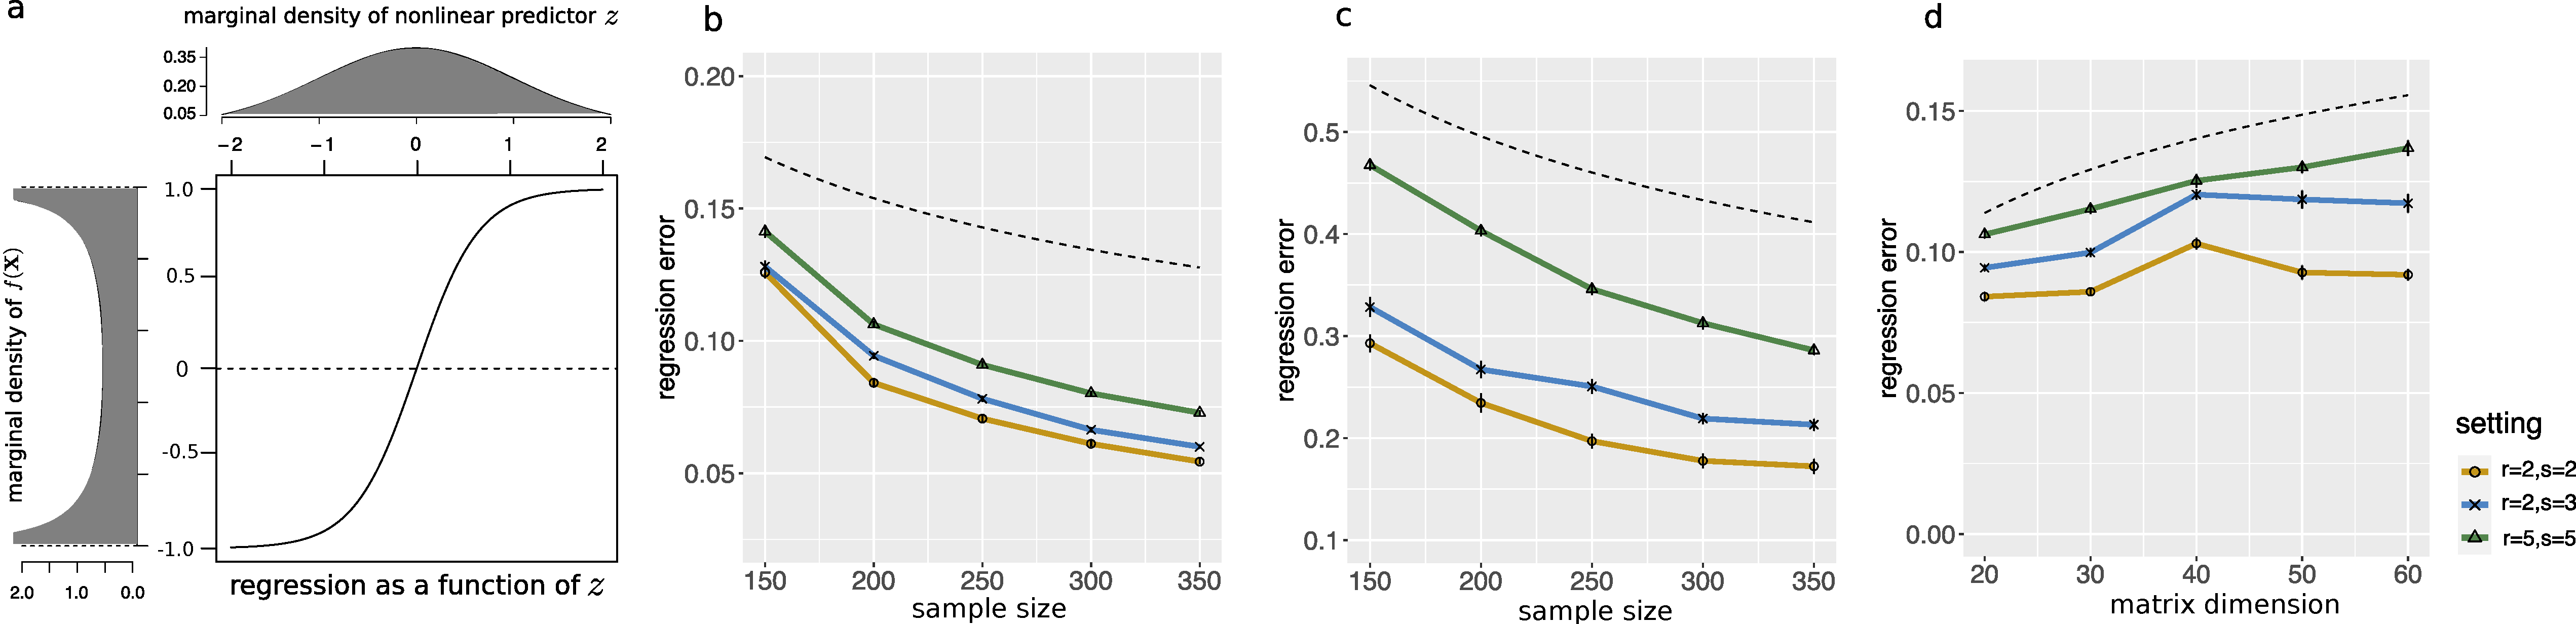
\includegraphics[width=\textwidth]{figure/combined_logistic.pdf}
\caption{Finite sample performance under a smooth function. (a) simulation setup; (b) prediction error with varying $n$ and $d=20$ for the continuous response; (c) for the binary response; (d) with varying $d$ and $n=200$. The dashed lines in panels (b)-(d) represent upper bounds $\tO(n^{-1/3})$, $\tO(n^{-1/3})$, and $\tO(\log d)$, respectively. The results are based on 30 data replications.} %, with standard error given in the error bar.}
\label{fig:logistic}
\end{figure}

The fourth experiment investigates the impact of smoothness in regression function. In Section~\ref{sec:idea}, we show that the probabilistic behavior of $f(\mX)$ plays a key role in our learning reduction approach. Here we assess the empirical performance by repeating all the above experiments using a model configuration with $z=z(\mX)\sim \text{Uniform}[-1,1]$, $h(z)=-0.6+1.2\mathds{1}(z>0)$, and $(r,s)=c(2,2),(2,5),(5,5)$. This case falls on the other end of the spectrum in contrast to the infinity smooth function in Fig~\ref{fig:logistic}(a). That is, $f(\mX)$ now concentrates at two mass points $\pi=\pm 0.6$. This makes the $\pi$-sign function estimation challenging around $\pi=\pm 0.6$ because of the non-identifiability. Figure \ref{fig:step} reports the new model configurations and the corresponding results. Interestingly, we find that our method still maintains good performance. One possible explanation of this robustness is that we aggregate in total $2H+1$ sign functions, each of which incurs at most $1/(2H+1)$ error to the regression function estimation. Therefore, our function estimate is robust against some off-target sign estimates, as long as the majority are accurate. This observation is consistent to the consistency result established in Section \ref{sec:bridge}.

\begin{figure}[t!]
\centering
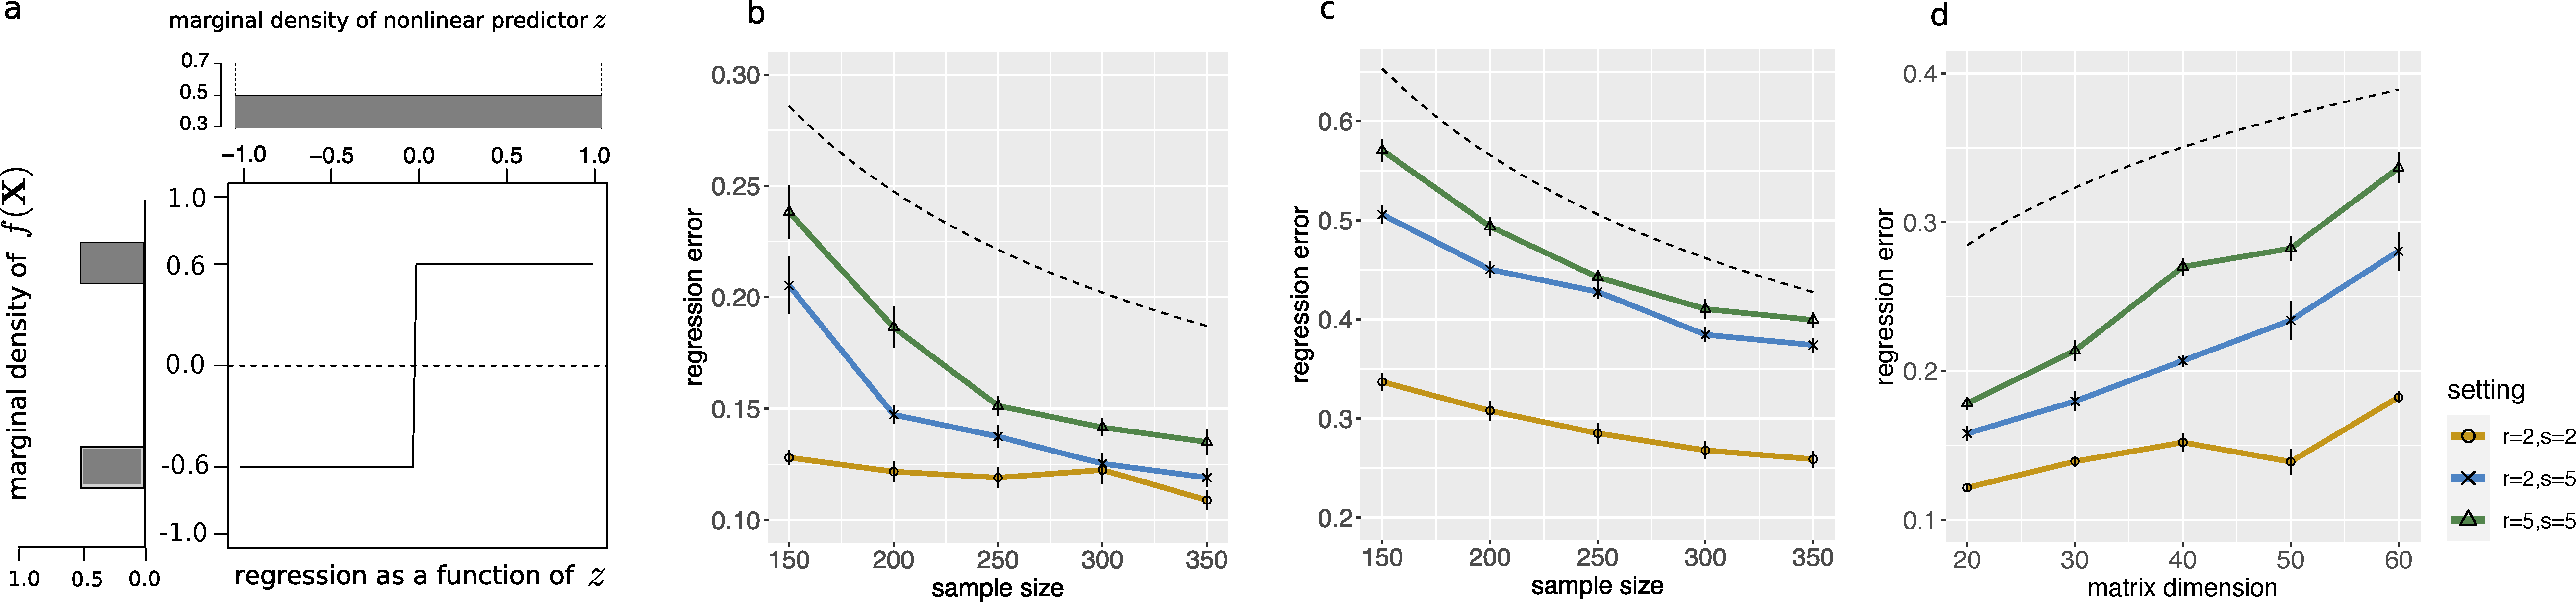
\includegraphics[width=\textwidth]{figure/combined_steps.pdf}
\caption{Finite sample performance under a non-smooth function. The setup is similar as Fig~\ref{fig:logistic}. The dashed lines in panels (b)-(d) represent upper bounds $\tO(n^{-1/2})$, $\tO(n^{-1/2})$, and $\tO(\log d)$, respectively.}
\label{fig:step}
\end{figure}



%%%%%%%%%%%%%%%%%%%%%%%%%%%%%%%%%%%%%%%%%%%%%%
\subsection{Comparison with alternative methods}
\label{sec:comparison}

Next, we compare our method with several popular alternative solutions. In this comparison, we adopt the simulation setup as in \cite{relion2019network}, but add more challenging matrix effects. Particularly, in this setup, the response is binary, and the predictor is a symmetric matrix that encodes a network. In this article, we have been targeting a general matrix predictor, which is directly applicable to a symmetric matrix, though we do not focus on symmetry. Moreover, as we show in Section~\ref{sec:joint} of the Appendix, the data generating model falls into our general family of nonparametric trace regression when there is no noise, but no longer so when there is noise. Therefore, we also investigate the performance of our method under model misspecification when including the noise. 

More specifically, we simulate from a latent variable model $(\mX,Y)|\pi$, where we generate $\pi$ i.i.d.\ from Uniform[0,1], and conditional on $\pi$, we generate $Y \sim \text{Bernoulli}(\pi)$, and 
\begin{eqnarray}\label{eq:pattern}
\mX=\entry{\mX_{ij}},\  \mX_{ij}\stackrel{\text{indep.}}{\sim} \text{Normal}\left( g_{ij}(\pi)\mathds{1}(\text{edge $(i,j)$ is active}), \sigma^2 \right), 
\end{eqnarray}
where the edge connectivity strength, denoted by $g_{ij}(\pi)$, varies depending on the location of $(i,j)\in[d]^2$, and the mean response $\pi$. Fig~\ref{fig:region} shows the activation pattern we consider that specifies the locations of the active edges. The active region is further divided into several subregions, each of which has its own signal function $g_{ij}(\cdot)\colon [0,1]\to \mathbb{R}$. The function form of $g_{ij}(\cdot)$ is randomly drawn from a pre-specified library consisting of common polynomial, log, and trigonometric functions. We set $d=68$, the training sample size $n=160$, and the testing size $80$. In the noiseless case $\sigma=0$ in~\eqref{eq:pattern}, the cross and block patterns are low-rank with $r = 3$ and 5, respectively, whereas the star and circle patterns are nearly full-rank, with a numerical rank $r \approx 30$ on the supported submatrix. 

\begin{figure}[t!]
\centering
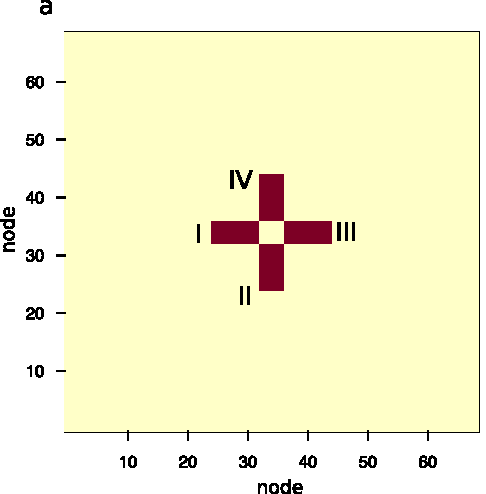
\includegraphics[width=3.3cm]{figure/cross.pdf}
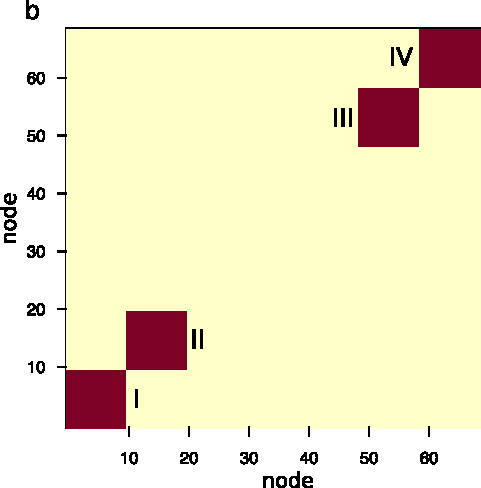
\includegraphics[width=3.3cm]{figure/block.pdf}
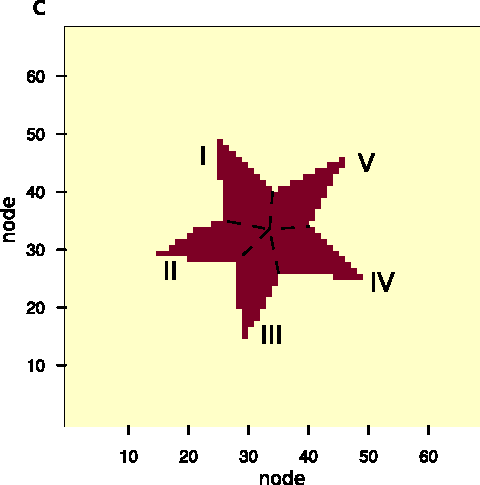
\includegraphics[width=3.3cm]{figure/star.pdf}
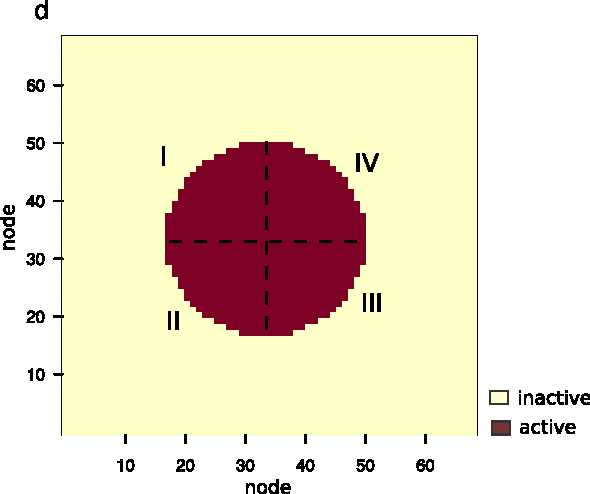
\includegraphics[width=4.1cm]{figure/circle.pdf}
\caption{Four activation patterns in simulations. The active region is divided into four or five subregions, denoted by I, II, ..., V, each of which has its own edge connectivity signal $g_{pq}(\pi)$.}
\label{fig:region}
\end{figure}

We compare the following four estimation methods. 

\begin{itemize}
\item Unstructured logistic regression for vector predictors ({\bf \footnotesize LogisticV}, \citep{Zou2005}). This method vectorizes the matrix predictor into a high-dimensional vector, then employs a logistic loss with an elastic net penalty. 

\item Generalized trace regression for matrix predictors ({\bf \footnotesize LogisticM},~\cite{relion2019network}). This method fits a parametric trace regression model with a logistic link and a symmetric matrix predictor. It imposes a group lasso penalty to encourage two-way sparsity. 

\item Convolutional Neural Network ({\bf \footnotesize CNN}) with two hidden layers implemented in Keras \cite{chollet2018deep}. We apply 64 filters with $3\times 3$ convolutional kernels to the matrix-valued predictor, followed by a pooling layer with size $5\times 5$. The resulting features are fed to a fully connected layer of neural network with ReLU activation. 

\item {\bf A}ggegration of {\bf S}tructured {\bf SI}gn {\bf S}eries for {\bf T}race regression ({\bf \footnotesize ASSIST}). This is our proposed method. 
\end{itemize}

\noindent 
Among these methods, \Lasso serves as a baseline to assess the gain of modeling a matrix predictor over a vector predictor, \LogisticM is a parametric model, whereas \CNN and \NonparaM are nonparametric solutions for matrix predictors. We feed each method with the binary response and the network adjacency matrix as the predictor after randomly permuting the node indices. Because \LogisticM only supports a symmetric matrix predictor, we provide it with $(\mX+\mX^T)/2$ as the input. We select the tuning parameters, including the rank $r$ and sparsity parameters $(r,s)$ for our method by 5-fold cross validation. We use the default parameters of \LogisticM, and select the tuning parameters of \Lasso and \CNN by 5-fold cross validation. 

\begin{figure}[b!]
\centering
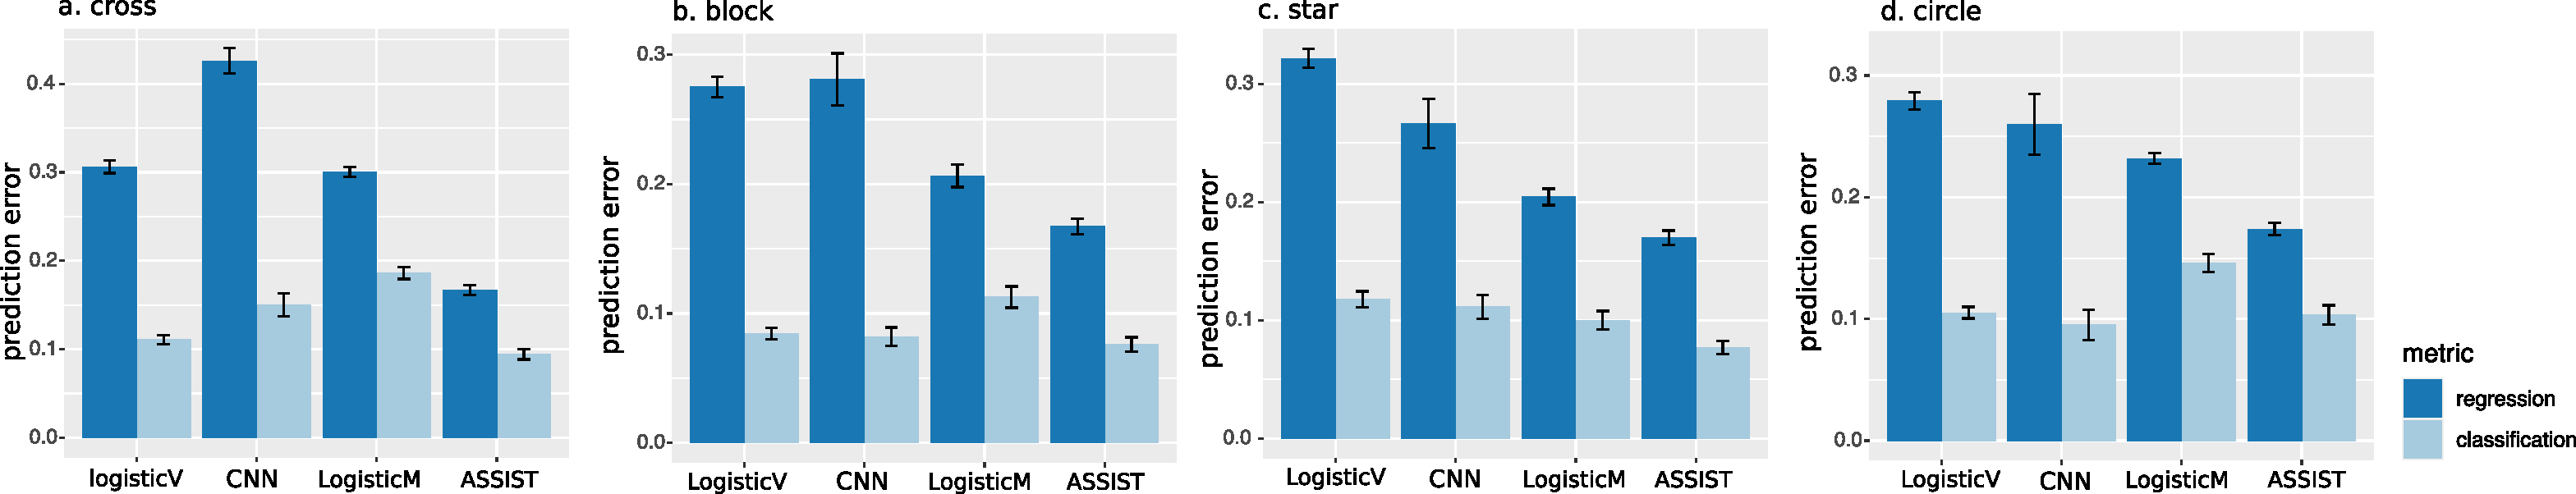
\includegraphics[width=\textwidth]{figure/error_tot_comb.pdf}
\caption{Performance comparison of various methods under four different activation patterns. Reported are the prediction error $\onenormSize{}{\hat f - f}$, denoted by ``regression",  and the misclassification error at $\pi=1/2$, denoted by ``classification". The results are based on 30 data replications.}
\label{fig:compare}
\end{figure}

Fig \ref{fig:compare} reports both the prediction error $\onenormSize{}{\hat f - f}$ and the misclassification error at $\pi=1/2$ of the four methods evaluated on the testing data. For the prediction performance, we see that \NonparaM consistently outperforms all of the alternative methods under comparison, and the improvement is substantial. For example, the relative reduction using \NonparaM over the next best approach, {\bf \footnotesize LogisticM}, is over 20\% for patterns (a) and (d), and over 15\% for patterns (b) and (c). The results clearly demonstrate
the benefit of our nonparametric approaches by allowing a more flexible functional form. Moreover, we find that neither \Lasso nor \CNN has satisfactory prediction performance. One possible reason is that these two methods fail to appropriately incorporate the network structure of the predictor. Particularly, \Lasso takes the vectorized matrix as the input and therefore loses the two-way pairing information. On the other hand, \CNN assumes spacial ordering within row and column indices. Although local similarity is important for the usual imaging analysis, the row and column indices take no particular order for a network. Actually, adjacency matrices after row or column permutation represent the same network, and thus the index-invariant methods, such as \LogisticM and \NonparaM, perform better. For the classification performance, we also see that our method overall performs the best. The only exception is the circle pattern where the \CNN has a slightly lower classification error. This is perhaps due to the fact that the circle pattern is nearly full rank which favors a more complicated model.  Interestingly, we also find that the advantage
of our method is more substantial in regression prediction than in classification, since classification is an easier problem than regression. Moreover, see that, with model noise included, our method still performs well even though the true model does not exactly follow our model specification. 

\begin{figure}[t!]
\centering
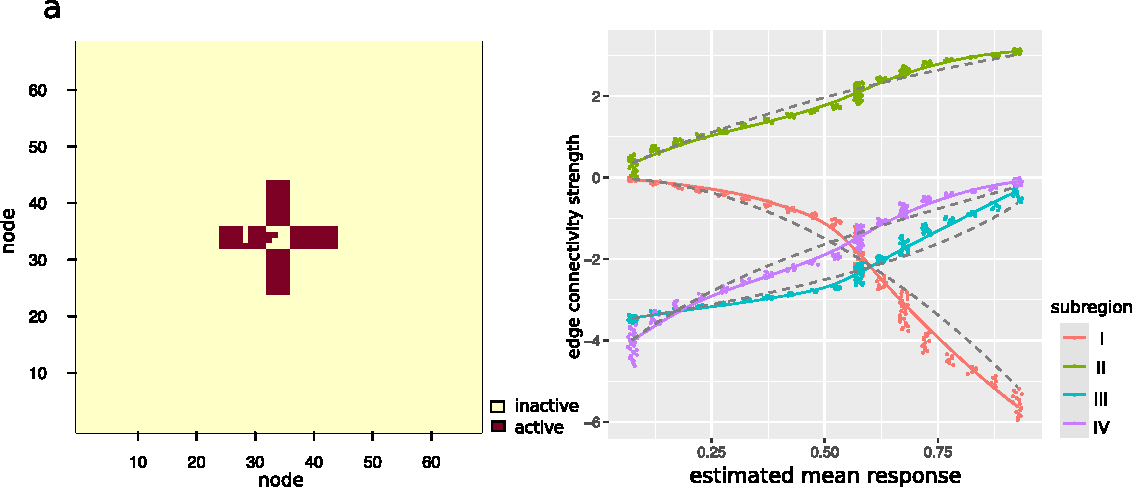
\includegraphics[width=7.05cm]{figure/est_cross.pdf} 
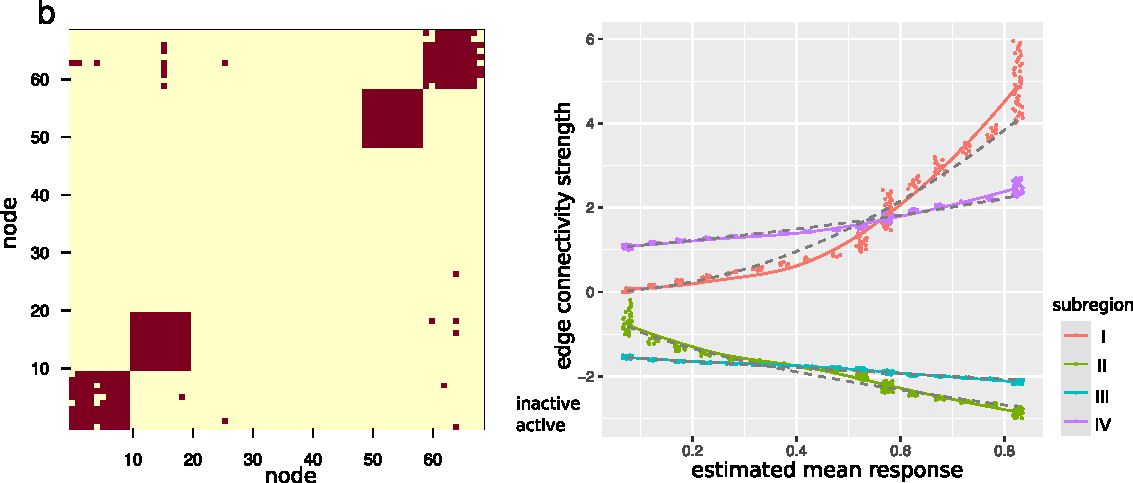
\includegraphics[width=7.05cm]{figure/est_block.pdf}
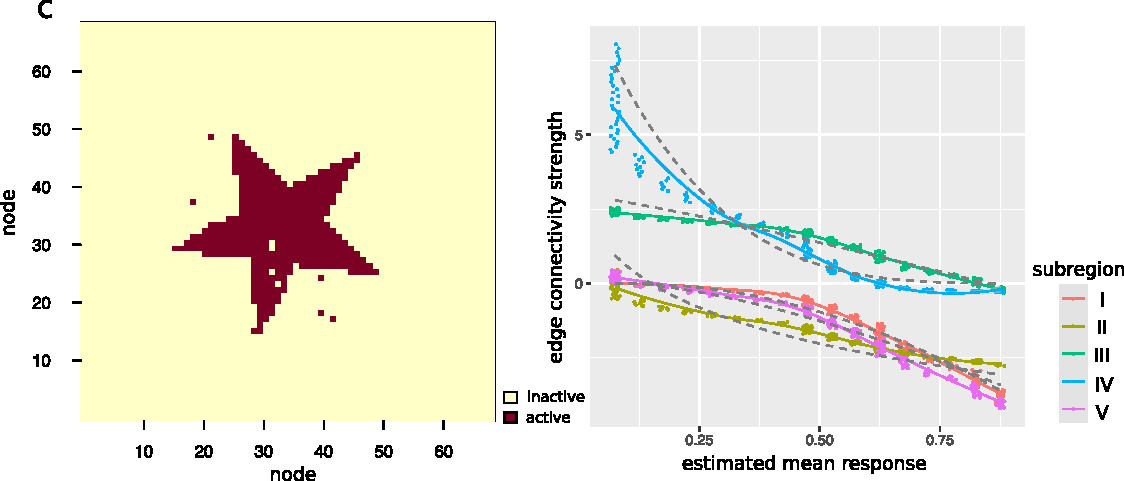
\includegraphics[width=7.05cm]{figure/est_star.pdf}
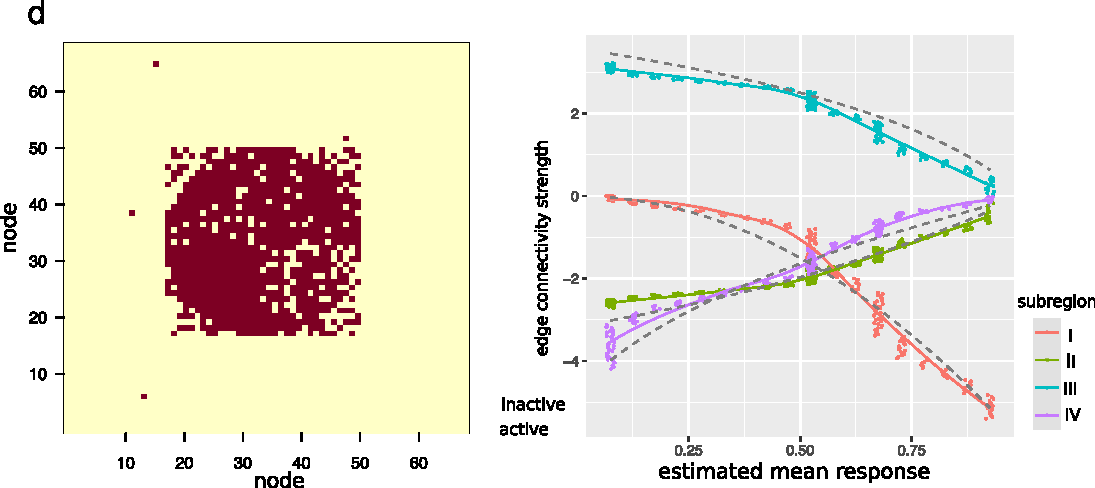
\includegraphics[width=7.05cm]{figure/est_circle.pdf}
\caption{Example output returned by {\bf \scriptsize ASSIST} based on the moving average of the feature weights, and the scatter plot of the edge connectivity strength, averaged by each subregion, versus the estimated mean response. The dashed curve shows the true function. }
\label{fig:compare2}
\end{figure}

Finally, to illustrate its capability of producing an estimate of high interpretability, Fig \ref{fig:compare2} reports the output of \NonparaM based on the moving average of the feature weights $(\hat \mB_\pi)_{\pi\in\Pi}$. It is observedthat the identified activation region agrees well with the truth. We also investigate the relationship between the edge connectivity for individual $i$ and the estimated mean response $\hat \pi_i$ for $i=1,\ldots,n$. The trajectory accurately resembles the ground truth function in each subregion, demonstrating that our method is able to recover the pattern in the matrix predictors $\mX_i$ against $\hat \pi_i$ on a continuous spectrum.





%%%%%%%%%%%%%%%%%%%%%%%%%%%%%%%%%%%%%%%%%%%%%%
\section{Real data applications}
\label{sec:realdata}

We present two real data applications, in parallel to the two matrix learning tasks studied in Section \ref{sec:examples}. The first task is binary-valued trait prediction based on brain connectivity matrix regression, and the second is continuous-valued matrix completion for imaging analysis. 



%%%%%%%%%%%%%%%%%%%%%%%%%%%%%%%%%%%%%%%%%%%%%%
\subsection{Brain connectivity analysis}
\label{sec:brain}

The first example is a brain connectivity data analysis, which aims to understand the relation between brain connectivity network and cognitive performance. The data is obtained from the Human Connectome Project (HCP) \cite{van2013wu}, and consists of $n=212$ healthy subjects. For each subject, a binary connectivity network is extracted, with nodes corresponding to $d=68$ brain regions-of-interest following the Desikan atlas \cite{desikan2006automated}, and links corresponding to the structural connectivity evaluated by diffusion tensor imaging \cite{zhang2018mapping}. The outcome is the dichotomized version of a visuospatial processing test score, corresponding to a high or low performance score \cite{wang2019common}. We adjust age and gender as additional covariates in our analysis. We note that, although our model focuses on a matrix predictor, it is straightforward to incorporate additional vector-valued covariates. We use a random 60-20-20 split of the data for training, validation, and testing. 

\begin{table}[t!]
\caption{Brain connectivity analysis. (a) Comparison of prediction accuracy measured by AUC, with standard errors over 5-fold cross validation in the parentheses. For \CNN, there is no report for node selection. (b) Top edges selected by the method {\footnotesize \bf ASSIST-p}. The letters ``r'' and ``l'' in node names indicate the right and left hemisphere, respectively. The $p$-value is calculated from the two-sample test of edge connection strength between two individual groups. }
\label{fig:real}
\resizebox{\columnwidth}{!}{
\begin{tabular}{ll}
a\hspace{6.5cm}b\\
\begin{tabular}{c|cc}
\hline
Method &  AUC  & \% of Active Nodes\\
\hline
{\bf \footnotesize ASSIST-p} &{\bf 0.73 (0.03)} &88.2   \\
{\bf \footnotesize ASSIST}& {\bf 0.77 (0.04)}  &97.3 \\
 LogisticM&0.72 (0.02)& 100.0\\
 LogisticV&0.68 (0.01)&89.7\\
CNN&0.67 (0.03)&-$^{}$\\
\hline
\end{tabular}
\begin{tabular}{c|ccc}
\hline
Rank &Node &  Node& $p$-value \\  
\hline
1&r-inferiortemporal&r-middletemporal&$0.01$\\
2&r-parstriangularis&r-supramarginal&3e-5\\
3&l-posteriorcingulate&r-precentral&0.01\\
4& l-caudalmiddlefronta& l-isthmuscingulate&2e-5\\
5 &l-lateralorbitofrontal&r-parstriangularis&1e-4\\
   \hline
\end{tabular}
\end{tabular}
}
\end{table}

\begin{figure}[b!]
\centering
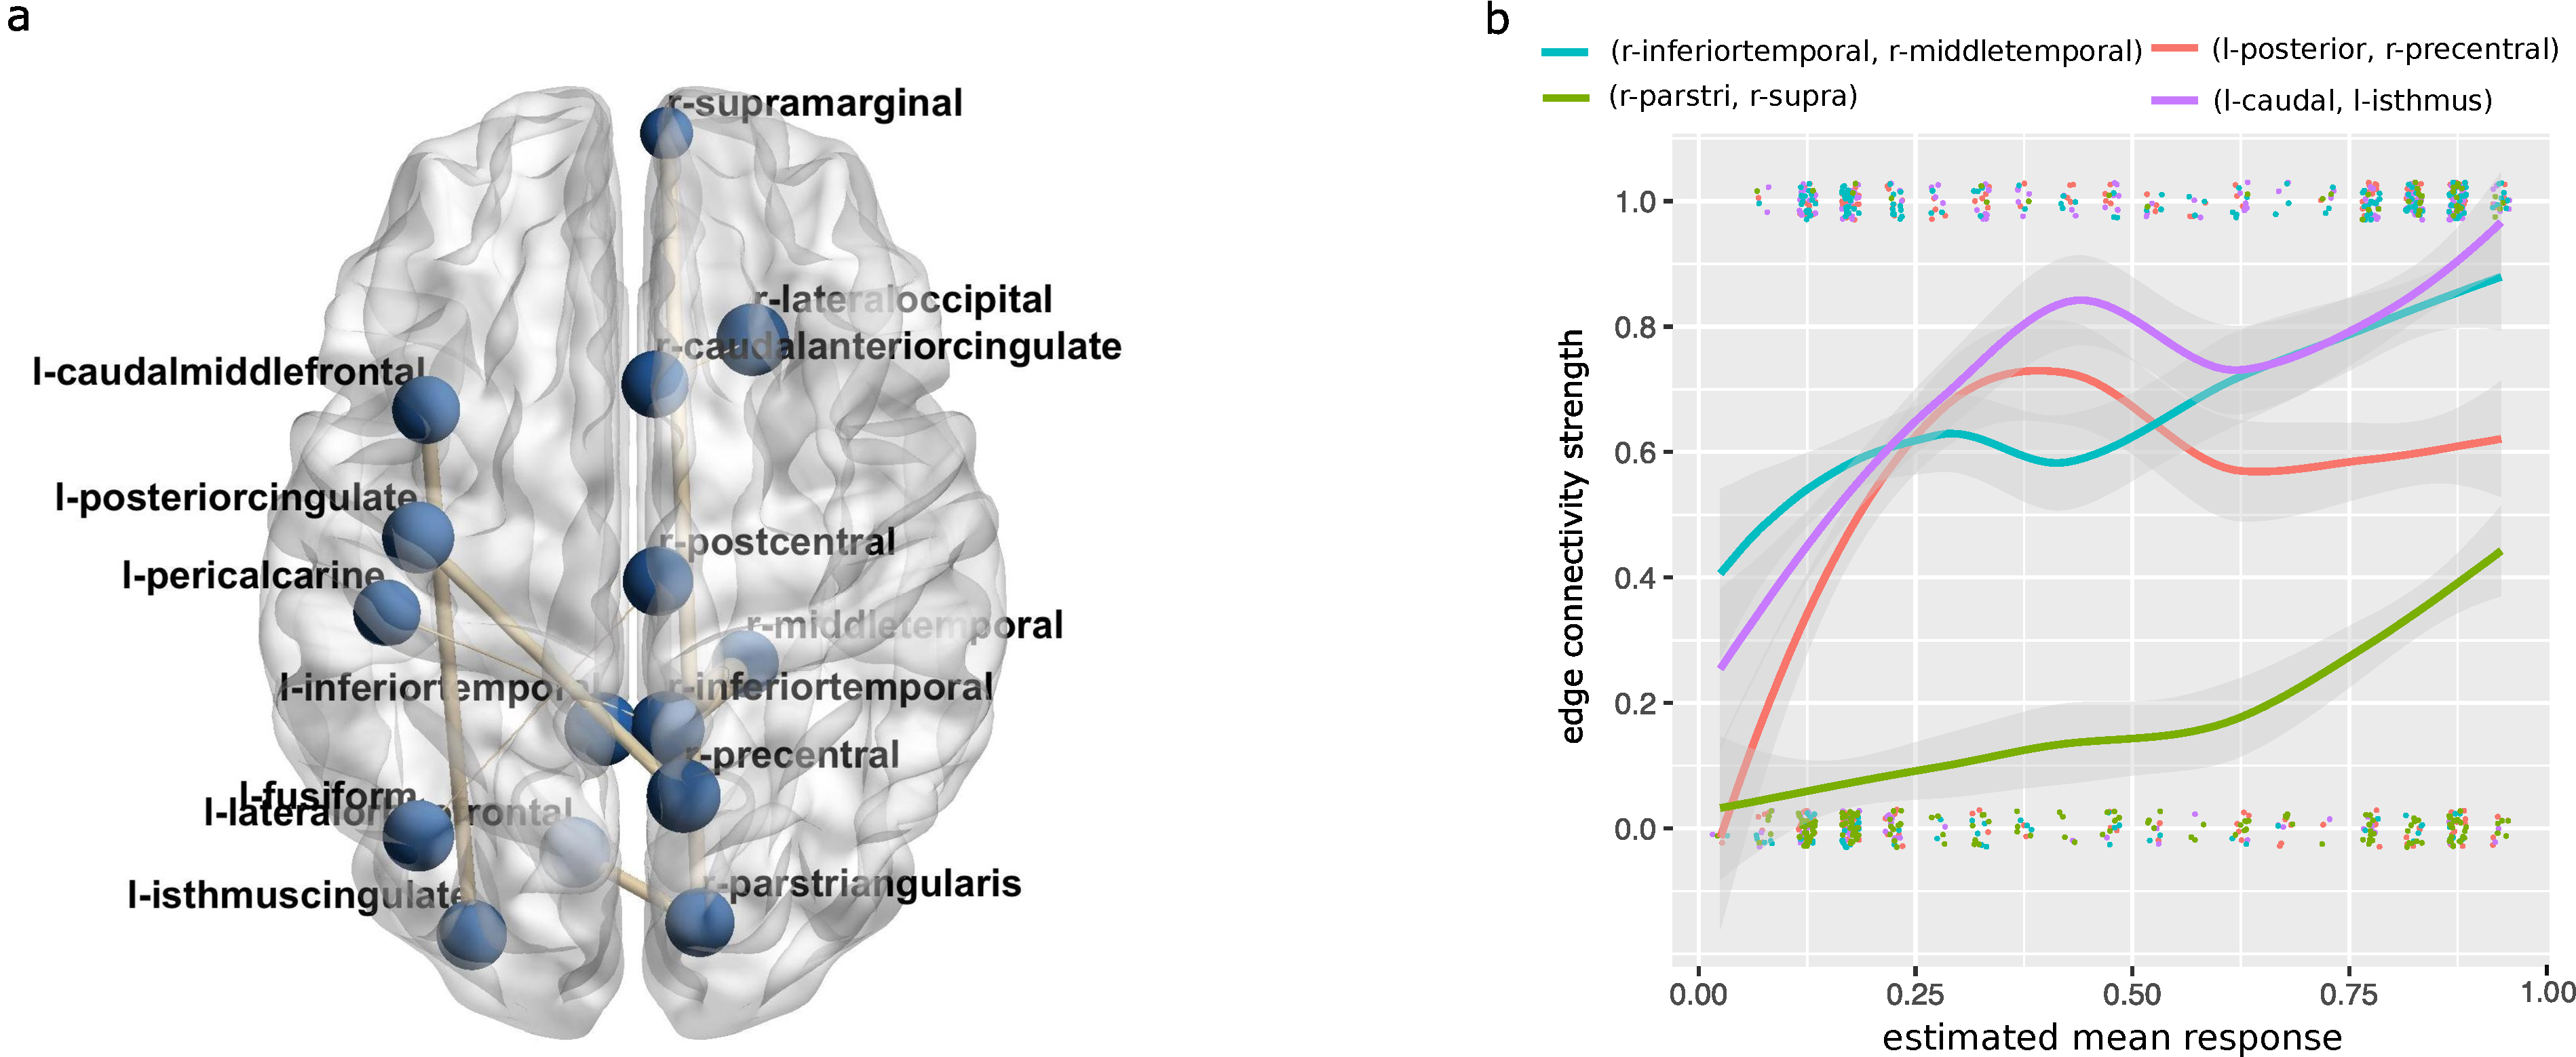
\includegraphics[width=.8\textwidth]{figure/brain.pdf}
\caption{Brain connectivity analysis.  (a) Top edges overlaid on a brain template. (b) Edge connectivity strength versus estimated mean response. Colored curves represent the moving averages of connectivity strengths, gray bands represent one standard error, and jitter points represent the raw connectivity values (0 or 1).}
\label{fig:real2}
\end{figure}

We compare our method with the same alternatives as in Section \ref{sec:comparison}. Table~\ref{fig:real}(a) shows that our method achieves the highest accuracy, measured by the area under receiver operating characteristic (AUC). Moreover, as common in the high-dimensional setting, we see the model with a good cross-validation accuracy tends to include a large number of noise variables. A useful heuristic called the ``one-standard-error rule'', suggested by \cite{hastie2015statistical}, selects the most parsimonious model with cross-validation accuracy within one standard error of the best. We apply this rule and report the results as {\bf \footnotesize ASSIST-p}. It is remarkable to see that {\bf \footnotesize ASSIST-p} results in 12\% reduction of active nodes but still achieves a comparable accuracy to the best one. Table~\ref{fig:real}(b) lists the top brain links identified by our method. The edges are ranked by their maximal values in the feature weights $(\hat \mB_\pi)_{\pi \in \tH}$ via moving averaging. We find that the top edges involve connections between frontal and occipital regions in the right hemisphere. This is consistent with recent findings of dysfunction in right posterior regions for deficits in visuospatial processing \cite{wang2019common}. Fig~\ref{fig:real2}(a) shows the top selected edges overlaid on a brain template. Moreover, we find the relationship between the edge connection strength and the mean response to be nonlinear. Fig~\ref{fig:real2}(b) plots the edge connectivity strength versus the estimated mean response. We see that the connection between r-parstriangularis and r-supramarginal grows slowly when the mean response is small but fast when it is large. In contrary, the connection between r-posteriorcingulate and r-precentral  grows fast initially, then reaches a plateau as the mean response increases. Such patterns suggest heterogeneous changes in brain connectivity with respect to the visuospatial processing capability. 



%%%%%%%%%%%%%%%%%%%%%%%%%%%%%%%%%%%%%%%%%%%%%%
\subsection{Imaging matrix completion}
\label{sec:completion}

The second application is an imaging matrix completion, where our goal is to recover and restore the partially observed gray-scaled hot air balloon image. This image is a standard benchmark in computer vision, and is organized as a 217-by-217 matrix, whose entries represent pixel values in $[0,1]$. We randomly mask a subset of entries and perform matrix completion based on the observed entries. 

We compare our method with three alternatives: a soft imputation method based on matrix nuclear norm regularization ({\bf \footnotesize SoftImpute})~\cite{hastie2015matrix}, a hard imputation method with ridge regression ({\bf \footnotesize HardImpute})~\cite{mazumder2010spectral}, and a hard imputation based on alternating SVD ({\bf \footnotesize Alt})~\cite{rennie2005fast}. We evaluate the recovery accuracy by MAE on the unobserved entries, and we tune all the parameters based on 5-fold cross-validation. 

\begin{figure}[h!]
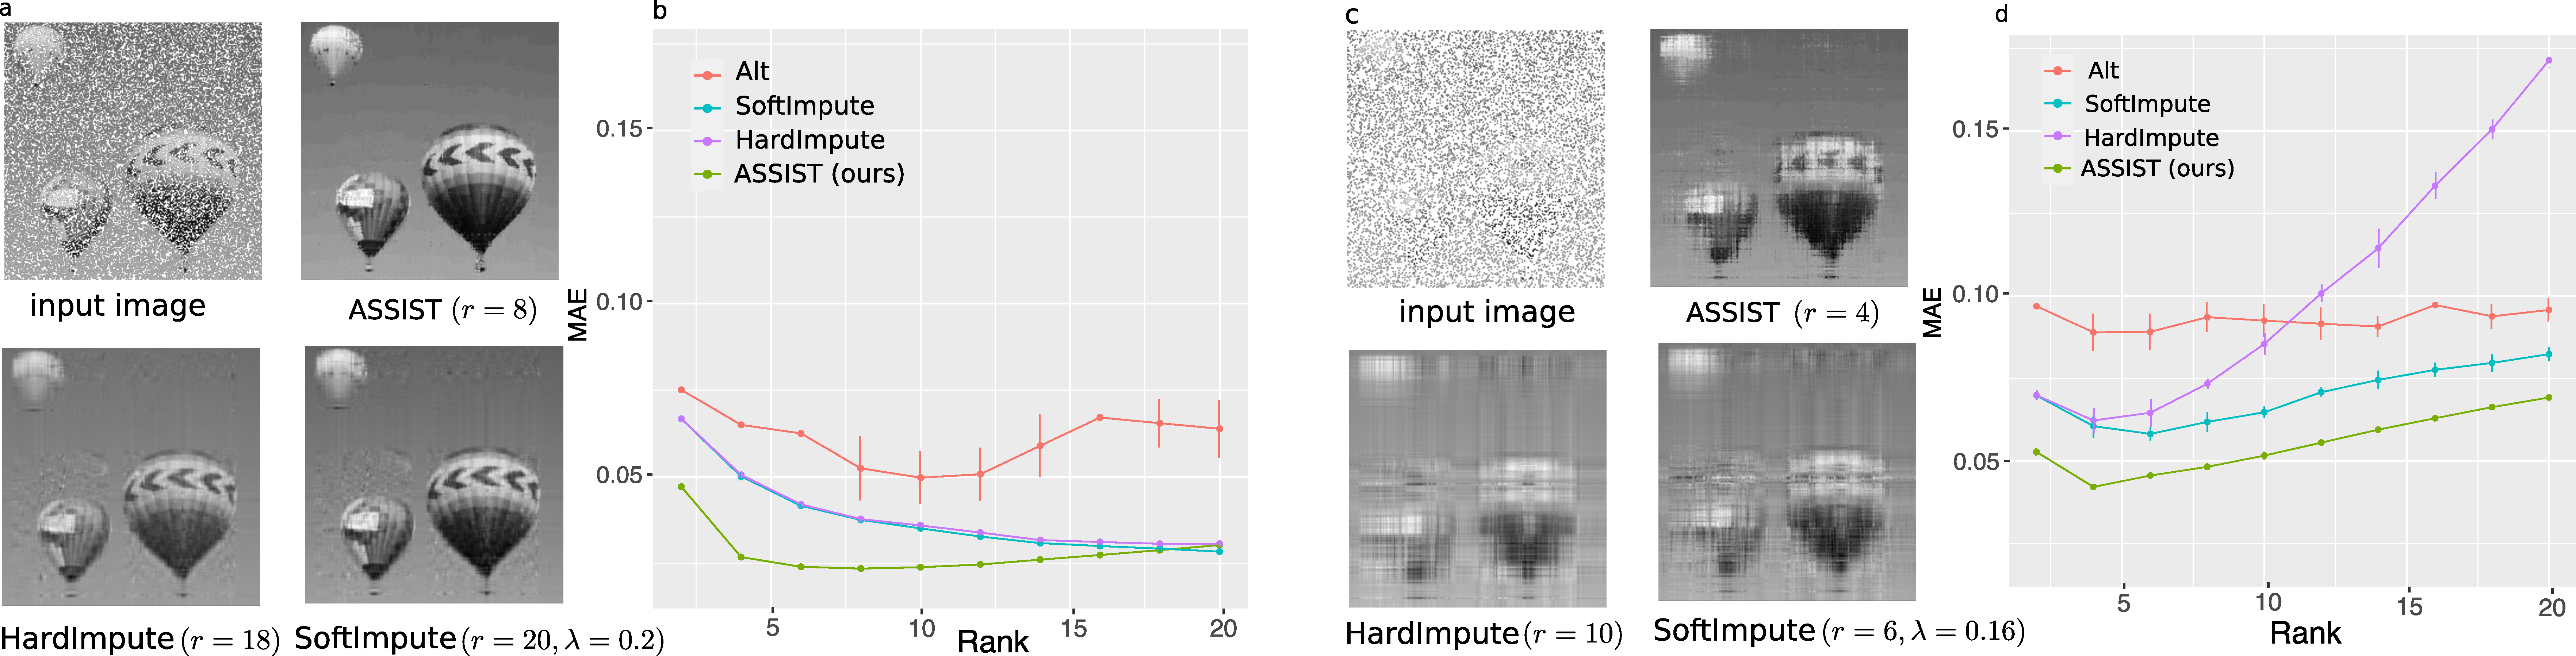
\includegraphics[width = \textwidth]{figure/completion.pdf}
\caption{Matrix completion analysis. (a)-(b) correspond to the 40\% missing rate, and (c)-(d) the 80\% missing rate. Error bars represent the standard error over 5-fold cross-validation. Numbers in the parentheses represent the selected tuning parameters for each method. In (a) and (c), we omit the worst method {\bf \scriptsize Alt} for space consideration.}
\label{fig:braincv}
\end{figure}

We investigate missing percentages at $40\%$ and $80\%$, and vary the rank $r=2,4,\ldots,20$. Fig \ref{fig:braincv} reports the performance comparison between four methods. We see clearly that our method achieves the best image recovery, with the smallest MAE. Besides, the advantage of our method compared to the alternative solutions is more clear when the missing percentage increases. 





%%%%%%%%%%%%%%%%%%%%%%%%%%%%%%%%%%%%%%%%%%%%%%
\section{Discussion}
\label{sec:discussion}

We have developed a nonparametric trace regression model for studying the relationship between a scalar response and a high-dimensional matrix predictor. We propose a learning reduction approach using structured sign function series, which bridges between regression and classification. We establish the theoretical bounds, which concern the fundamental statistical errors, are independent of specific algorithms, and serve as a benchmark on how well any algorithmic procedure could perform. Our numerical results demonstrate the competitive performance of the proposed method.

Our work unlocks several possible future directions. One is nonparametric modeling of other nonconventional predictors, such as tensors, functions, and manifold data. Another direction includes multi-task learning and compressed sensing. Moreover, our learning reduction approach can be coupled with more sophisticated classifiers, such as neural networks, decision trees, and boosting, for sign function estimation. Finally, the theoretical guarantees we obtain are for the global optimum. How to characterize the behavior of the actual minimizer, or relatedly, the computational error for non-convex matrix-based regression remains challenging and open. All these questions are warranted for future research. 





%%%%%%%%%%%%%%%%%%%%%%%%%%%%%%%%%%%%%%%%%%%%%%
%\section*{Acknowledgements}
%The authors would like to thank the anonymous referees, an Associate Editor and the Editor for their constructive comments that improved the quality of this paper.





%%%%%%%%%%%%%%%%%%%%%%%%%%%%%%%%%%%%%%%%%%%%%%
\begin{supplement}
%\stitle{Supplementary Material}
%\sdescription{}
Supplementary Appendix includes all technical proofs and additional results. Our software {\bf \footnotesize ASSIST} and data used in our analysis are publicly available at \url{https://github.com/Miaoyanwang/nonparametric}.
\end{supplement}





%%%%%%%%%%%%%%%%%%%%%%%%%%%%%%%%%%%%%%%%%%%%%%
\bibliographystyle{imsart-number} 
\bibliography{ref-trace}       





\end{document}
